% Adapted from Emily's dissertation template
\documentclass[phd]{nuthesis}
\usepackage{amssymb, amsmath, amsfonts}
\usepackage{calc}
\usepackage{graphicx}
\usepackage[hidelinks]{hyperref}
\usepackage{indentfirst}
\makeatletter
\def\maxwidth{\ifdim\Gin@nat@width>\linewidth\linewidth\else\Gin@nat@width\fi}
\def\maxheight{\ifdim\Gin@nat@height>\textheight\textheight\else\Gin@nat@height\fi}
\makeatother
\setkeys{Gin}{width=\maxwidth,height=\maxheight,keepaspectratio}

\usepackage{color}
\usepackage{fancyvrb}
\newcommand{\VerbBar}{|}
\newcommand{\VERB}{\Verb[commandchars=\\\{\}]}
\DefineVerbatimEnvironment{Highlighting}{Verbatim}{commandchars=\\\{\}}
% Add ',fontsize=\small' for more characters per line
\usepackage{framed}
\definecolor{shadecolor}{RGB}{241,243,245}
\newenvironment{Shaded}{\begin{snugshade}}{\end{snugshade}}
\newcommand{\AlertTok}[1]{\textcolor[rgb]{0.68,0.00,0.00}{#1}}
\newcommand{\AnnotationTok}[1]{\textcolor[rgb]{0.37,0.37,0.37}{#1}}
\newcommand{\AttributeTok}[1]{\textcolor[rgb]{0.40,0.45,0.13}{#1}}
\newcommand{\BaseNTok}[1]{\textcolor[rgb]{0.68,0.00,0.00}{#1}}
\newcommand{\BuiltInTok}[1]{\textcolor[rgb]{0.00,0.23,0.31}{#1}}
\newcommand{\CharTok}[1]{\textcolor[rgb]{0.13,0.47,0.30}{#1}}
\newcommand{\CommentTok}[1]{\textcolor[rgb]{0.37,0.37,0.37}{#1}}
\newcommand{\CommentVarTok}[1]{\textcolor[rgb]{0.37,0.37,0.37}{\textit{#1}}}
\newcommand{\ConstantTok}[1]{\textcolor[rgb]{0.56,0.35,0.01}{#1}}
\newcommand{\ControlFlowTok}[1]{\textcolor[rgb]{0.00,0.23,0.31}{\textbf{#1}}}
\newcommand{\DataTypeTok}[1]{\textcolor[rgb]{0.68,0.00,0.00}{#1}}
\newcommand{\DecValTok}[1]{\textcolor[rgb]{0.68,0.00,0.00}{#1}}
\newcommand{\DocumentationTok}[1]{\textcolor[rgb]{0.37,0.37,0.37}{\textit{#1}}}
\newcommand{\ErrorTok}[1]{\textcolor[rgb]{0.68,0.00,0.00}{#1}}
\newcommand{\ExtensionTok}[1]{\textcolor[rgb]{0.00,0.23,0.31}{#1}}
\newcommand{\FloatTok}[1]{\textcolor[rgb]{0.68,0.00,0.00}{#1}}
\newcommand{\FunctionTok}[1]{\textcolor[rgb]{0.28,0.35,0.67}{#1}}
\newcommand{\ImportTok}[1]{\textcolor[rgb]{0.00,0.46,0.62}{#1}}
\newcommand{\InformationTok}[1]{\textcolor[rgb]{0.37,0.37,0.37}{#1}}
\newcommand{\KeywordTok}[1]{\textcolor[rgb]{0.00,0.23,0.31}{\textbf{#1}}}
\newcommand{\NormalTok}[1]{\textcolor[rgb]{0.00,0.23,0.31}{#1}}
\newcommand{\OperatorTok}[1]{\textcolor[rgb]{0.37,0.37,0.37}{#1}}
\newcommand{\OtherTok}[1]{\textcolor[rgb]{0.00,0.23,0.31}{#1}}
\newcommand{\PreprocessorTok}[1]{\textcolor[rgb]{0.68,0.00,0.00}{#1}}
\newcommand{\RegionMarkerTok}[1]{\textcolor[rgb]{0.00,0.23,0.31}{#1}}
\newcommand{\SpecialCharTok}[1]{\textcolor[rgb]{0.37,0.37,0.37}{#1}}
\newcommand{\SpecialStringTok}[1]{\textcolor[rgb]{0.13,0.47,0.30}{#1}}
\newcommand{\StringTok}[1]{\textcolor[rgb]{0.13,0.47,0.30}{#1}}
\newcommand{\VariableTok}[1]{\textcolor[rgb]{0.07,0.07,0.07}{#1}}
\newcommand{\VerbatimStringTok}[1]{\textcolor[rgb]{0.13,0.47,0.30}{#1}}
\newcommand{\WarningTok}[1]{\textcolor[rgb]{0.37,0.37,0.37}{\textit{#1}}}

\makeatletter
\@ifpackageloaded{bookmark}{}{\usepackage{bookmark}}
\makeatother
\makeatletter
\@ifpackageloaded{caption}{}{\usepackage{caption}}
\AtBeginDocument{%
\ifdefined\contentsname
  \renewcommand*\contentsname{Table of contents}
\else
  \newcommand\contentsname{Table of contents}
\fi
\ifdefined\listfigurename
  \renewcommand*\listfigurename{List of Figures}
\else
  \newcommand\listfigurename{List of Figures}
\fi
\ifdefined\listtablename
  \renewcommand*\listtablename{List of Tables}
\else
  \newcommand\listtablename{List of Tables}
\fi
\ifdefined\figurename
  \renewcommand*\figurename{Figure}
\else
  \newcommand\figurename{Figure}
\fi
\ifdefined\tablename
  \renewcommand*\tablename{Table}
\else
  \newcommand\tablename{Table}
\fi
}
\@ifpackageloaded{float}{}{\usepackage{float}}
\floatstyle{ruled}
\@ifundefined{c@chapter}{\newfloat{codelisting}{h}{lop}}{\newfloat{codelisting}{h}{lop}[chapter]}
\floatname{codelisting}{Listing}
\newcommand*\listoflistings{\listof{codelisting}{List of Listings}}
\makeatother
\makeatletter
\makeatother
\makeatletter
\@ifpackageloaded{caption}{}{\usepackage{caption}}
\@ifpackageloaded{subcaption}{}{\usepackage{subcaption}}
\makeatother

\newlength{\cslhangindent}
\setlength{\cslhangindent}{1.5em}
\newlength{\csllabelwidth}
\setlength{\csllabelwidth}{3em}
\newenvironment{CSLReferences}[2]
 {\begin{thebibliography}{999}
	\setlength{\itemsep}{#2\baselineskip}}
 {\end{thebibliography}}
\newcommand{\citeproctext}{}
\newcommand{\CSLBlock}[1]{#1\hfill\break}
\newcommand{\CSLLeftMargin}[1]{\parbox[t]{\csllabelwidth}{#1}}
\newcommand{\CSLRightInline}[1]{\parbox[t]{\linewidth - \csllabelwidth}{#1}\break}
\newcommand{\CSLIndent}[1]{\hspace{\cslhangindent}#1}

\title{Perception of 3D Data Visualizations}
\author{Tyler Wiederich}

\AtBeginDocument{\frontmatter}
\geometry{letterpaper,top=1in,bottom=1in,right=1in,left=1.5in,includehead,nofoot}
\AtBeginDocument{\raggedright}
\AtBeginDocument{%
	\setlength{\parindent}{2em}%
	\setlength{\parskip}{0pt}%
}

\major{Statistics}
\adviser{Professor Susan VanderPlas}
\adviserAbstract{Susan VanderPlas}
\degreemonth{August}
\degreeyear{2026}

\begin{document}
\maketitle

\begin{abstract}
Data visualizations are a powerful tool for the communication of complex
data structures.

Lorem ipsum dolor sit amet, consectetur adipiscing elit. Sed do eiusmod
tempor incididunt ut labore et dolore magna aliqua. Ut enim ad minim
veniam, quis nostrud exercitation ullamco laboris nisi ut aliquip ex ea
commodo consequat.

Duis aute irure dolor in reprehenderit in voluptate velit esse cillum
dolore eu fugiat nulla pariatur. Excepteur sint occaecat cupidatat non
proident, sunt in culpa qui officia deserunt mollit anim id est laborum.
\end{abstract}

\begin{acknowledgments}
A section to thank those who have supported my research and academic
journey!
\end{acknowledgments}

\setcounter{tocdepth}{1}
\tableofcontents
\listoffigures
\listoftables

\mainmatter

\bookmarksetup{startatroot}

\chapter{Literature Review}\label{literature-review}

\section{Motivation and Background}\label{motivation-and-background}

Data visualizations play an essential role in understanding patterns in
the structure of data. They allow for a programmatic mapping of data
into a ``picture'' that can be used to gather insight from the viewer
(Tufte, 2001; Tukey, 1965; Wilkinson \& Wills, 2005). Since the early
20th century, researchers have been exploring the question: what makes a
good graph? (Cleveland \& McGill, 1984; Croxton \& Stein, 1932; Croxton
\& Stryker, 1927; Vanderplas et al., 2020). Many attempts to answer this
question have provided good recommendations, but are largely limited to
the projection of graphs onto 2-dimensional (2D) surfaces. While this
addresses many of the typical use cases for data visualizations, the
process of creating modern statistical graphics in our 3-dimensional
(3D) world is a relatively new phenomenon that does not have widespread
usage (Huron et al., 2023).

Many charts exist within the confines of a 2D projected space due to the
practicality of computer renderings. These computer-generated graphics
are quick and cheap to produce (Tukey, 1965), which possibly contributes
to their widespread usage. Before computers, hand-drawn and complex
printing techniques were common production methods and took time to
produce (Friendly \& Wainer, 2021; VanderPlas et al., 2019). In
contrast, all data physicalizations require additional material
resources, increasing the base cost to produce. Additionally, there are
few modern resources that have direct pipelines from data to physical
objects. One such example is the \texttt{rayshader} package
(Morgan-Wall, 2024), although modifications to the resulting
stereolithography (STL) file or OBJ file are needed before
physicalization can take place. The cost and lack of tools for producing
physical charts likely results in the majority of modern graphics being
produced with 2D representations on digital screens.

Nearly every type of chart can be created by using a programmatic
mapping of data and variables to aesthetics and geometries, a process
sometimes referred to as the ``Grammar of Graphics'' (Wilkinson \&
Wills, 2005). This has found widespread implementation into numerous
software (\emph{SAS 9.4 ODS Graphics}, n.d.; Satyanarayan et al., 2017;
Wickham, 2010). For example, consider the chart created in
Figure~\ref{fig-quick-plot}. In this figure, the Palmer Penguins dataset
(Horst et al., 2020) is supplied to the \texttt{ggplot} function from
the \texttt{ggplot2} package (Wickham, 2016). The x and y axes are
mapped to bill length and bill depth, with color and shape being mapped
to island. The geometry is given by \texttt{geom\_point}, which results
in a scatterplot that shows each complete data observation. Although the
chart would benefit from further customization, it was quick to produce
and has instant visual insights. Other software packages can create the
same chart using a similar process by specifying the axes, colors, and
shapes using a point geometry.

\newpage

\begin{Shaded}
\begin{Highlighting}[]
\FunctionTok{library}\NormalTok{(tidyverse)}
\FunctionTok{library}\NormalTok{(palmerpenguins)}
\FunctionTok{ggplot}\NormalTok{(penguins, }\AttributeTok{mapping =} \FunctionTok{aes}\NormalTok{(}\AttributeTok{x =}\NormalTok{ bill\_length\_mm, }
                               \AttributeTok{y =}\NormalTok{ bill\_depth\_mm, }
                               \AttributeTok{color =}\NormalTok{ island, }
                               \AttributeTok{shape =}\NormalTok{ island)) }\SpecialCharTok{+} 
  \FunctionTok{geom\_point}\NormalTok{()}
\end{Highlighting}
\end{Shaded}

\begin{figure}[H]

\centering{

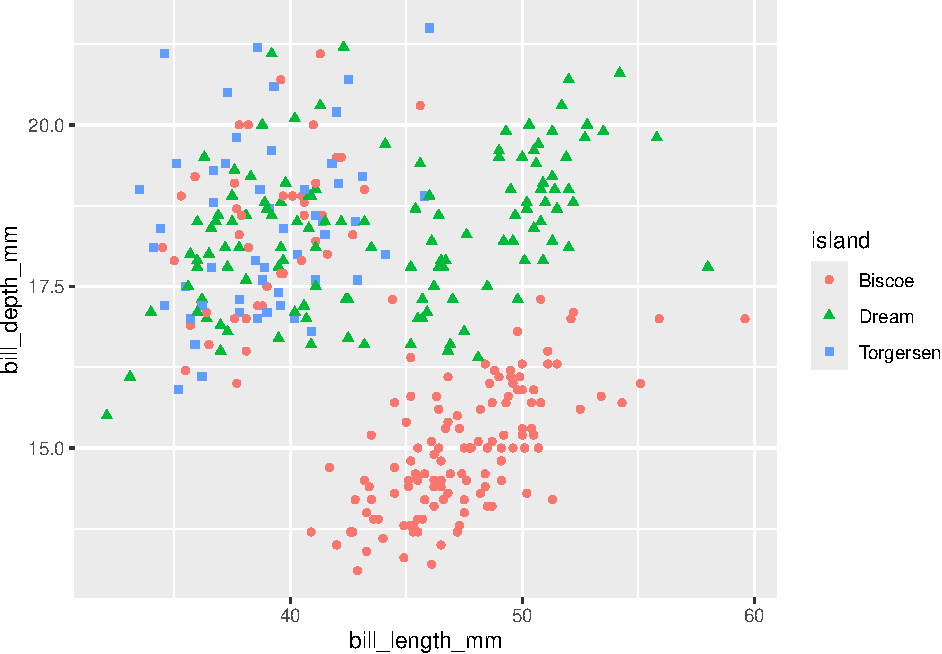
\includegraphics{index_files/figure-pdf/fig-quick-plot-1.pdf}

}

\caption[Grammar of graphics example]{\label{fig-quick-plot}Penguins
dataset (Horst et al., 2020) showing the construction of a plot using
\texttt{ggplot2} in R.}

\end{figure}%

While there have been many attempts to establish good data visualization
practices (Tufte, 2001; Vanderplas et al., 2020), we do not know how
well these recommendations translate from 2D projections into our 3D
world. The advent of 3D printing allows us to precisely construct the 3D
charts that have been widely studied through their 2D representations
(Barfield \& Robless, 1989; Croxton \& Stein, 1932; Zacks et al., 1998).
With limited research on 3D-printed data manifestations, we explore some
of the first empirical findings of physical 3D statistical graphics.

\section{Overview of Physical 3D
Visualizations}\label{overview-of-physical-3d-visualizations}

Data can be expressed in the physical world through a wide variety of
means. In many cases, this can take on artistic expressions, such as
encoding information into crocheted blankets or wooden sculptures (Huron
et al., 2023). While certainly providing information about the data,
these informational art pieces are largely left as display items to
promote conversation into the underlying dataset.

\begin{figure}

\centering{

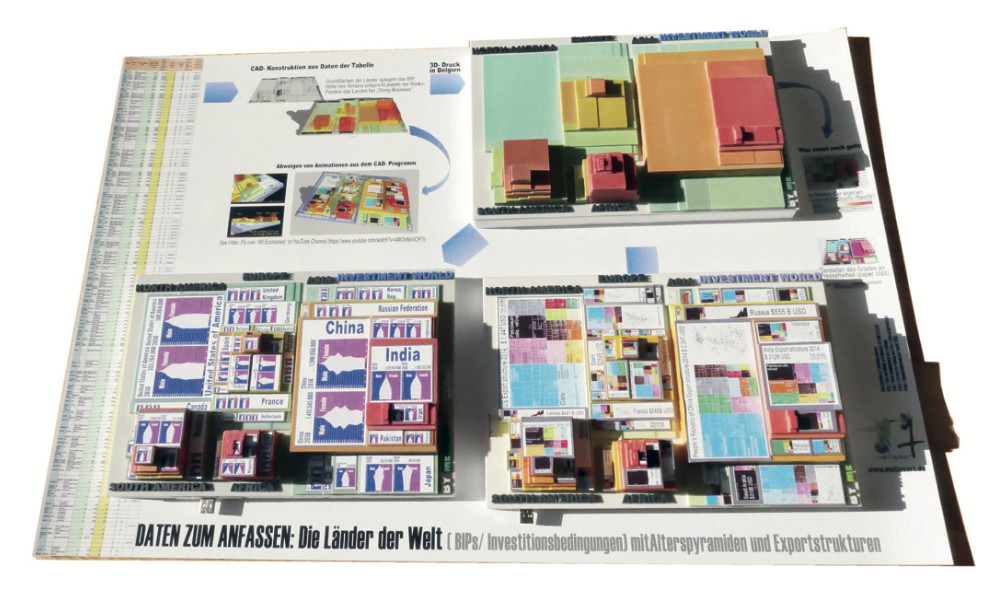
\includegraphics[width=0.8\textwidth,height=\textheight]{images/treemap-3d.png}

}

\caption[3D-printed treemap]{\label{fig-3d-treemap}3D-printed treemap
created displaying Gross National Income for 130 countries (Huron et
al., 2023, pg. 217). The two 3D prints on the bottom have additional
information overlaid on top of the treemap as 2D displays.}

\end{figure}%

Perhaps one of the most affordable types of data physicalization is
through the use of 3D printing. Aside from the startup cost of a
3D-printer, material and labor costs are relatively low. Rolls of PLA
filament can be acquired for around \$20 and can be used to create
multiple charts. Print times vary depending on the size and complexity
of the graphic, but smaller charts can be produced in approximately 2
hours. While needing much more time to produce than computer-generated
visualizations, the amount of hands-on labor during the 3D-printing
process is mainly limited to the time it takes to create the print file.

Using 3D printers to create statistical graphics has typically been
reserved for niche purposes to promote engagement of the displayed data.
One of the earliest 3D-printed charts was shared in 2014 by the Wall
Street Journal, where the print was used to discuss the rising
popularity of 3D printers (Thingiverse.com, n.d.;
\textbf{graphicsHowDoes3D?}). It is rare to find these types of charts
in practice, where images of the charts are often posted to social media
or blog posts. This results in limited access to the physical charts,
even though source print files can be shared through sites such as
\url{thingiverse.com} and \url{printables.com}, as well as through
GitHub.

\begin{figure}

\begin{minipage}{\linewidth}

\centering{

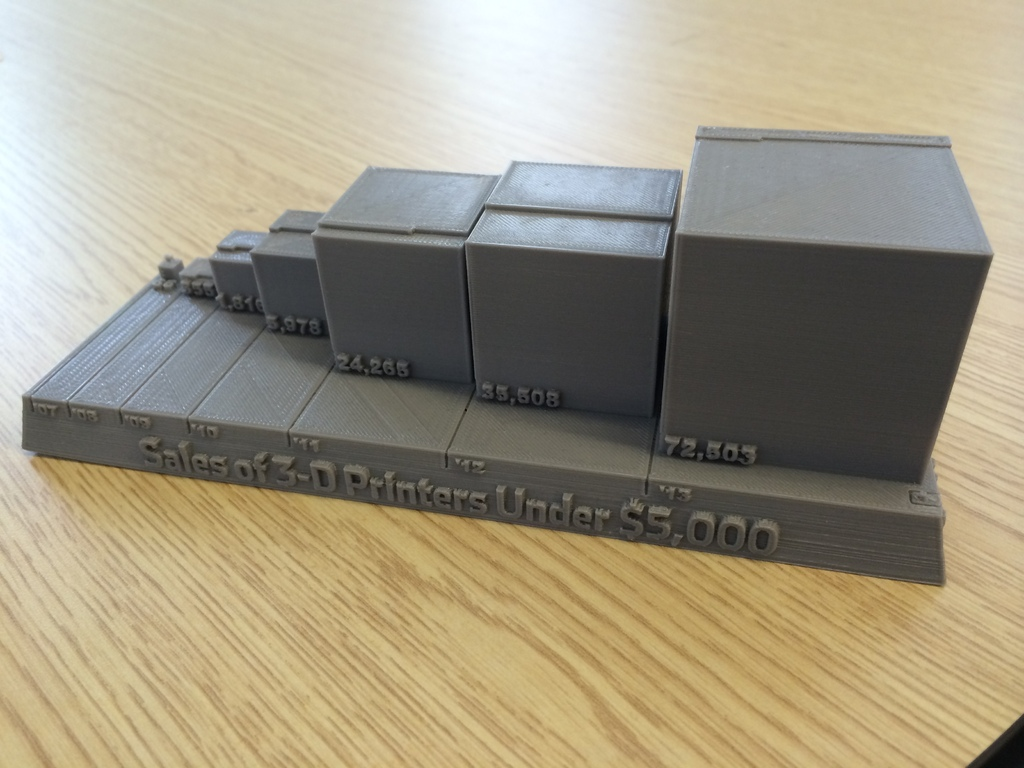
\includegraphics[width=\textwidth,height=2in]{images/wsj-print.jpg}

}

\subcaption[Original WSJ 3D print]{\label{fig-wsj-orig}Original 3D
printed chart from WSJ}

\end{minipage}%
\newline
\begin{minipage}{\linewidth}

\centering{

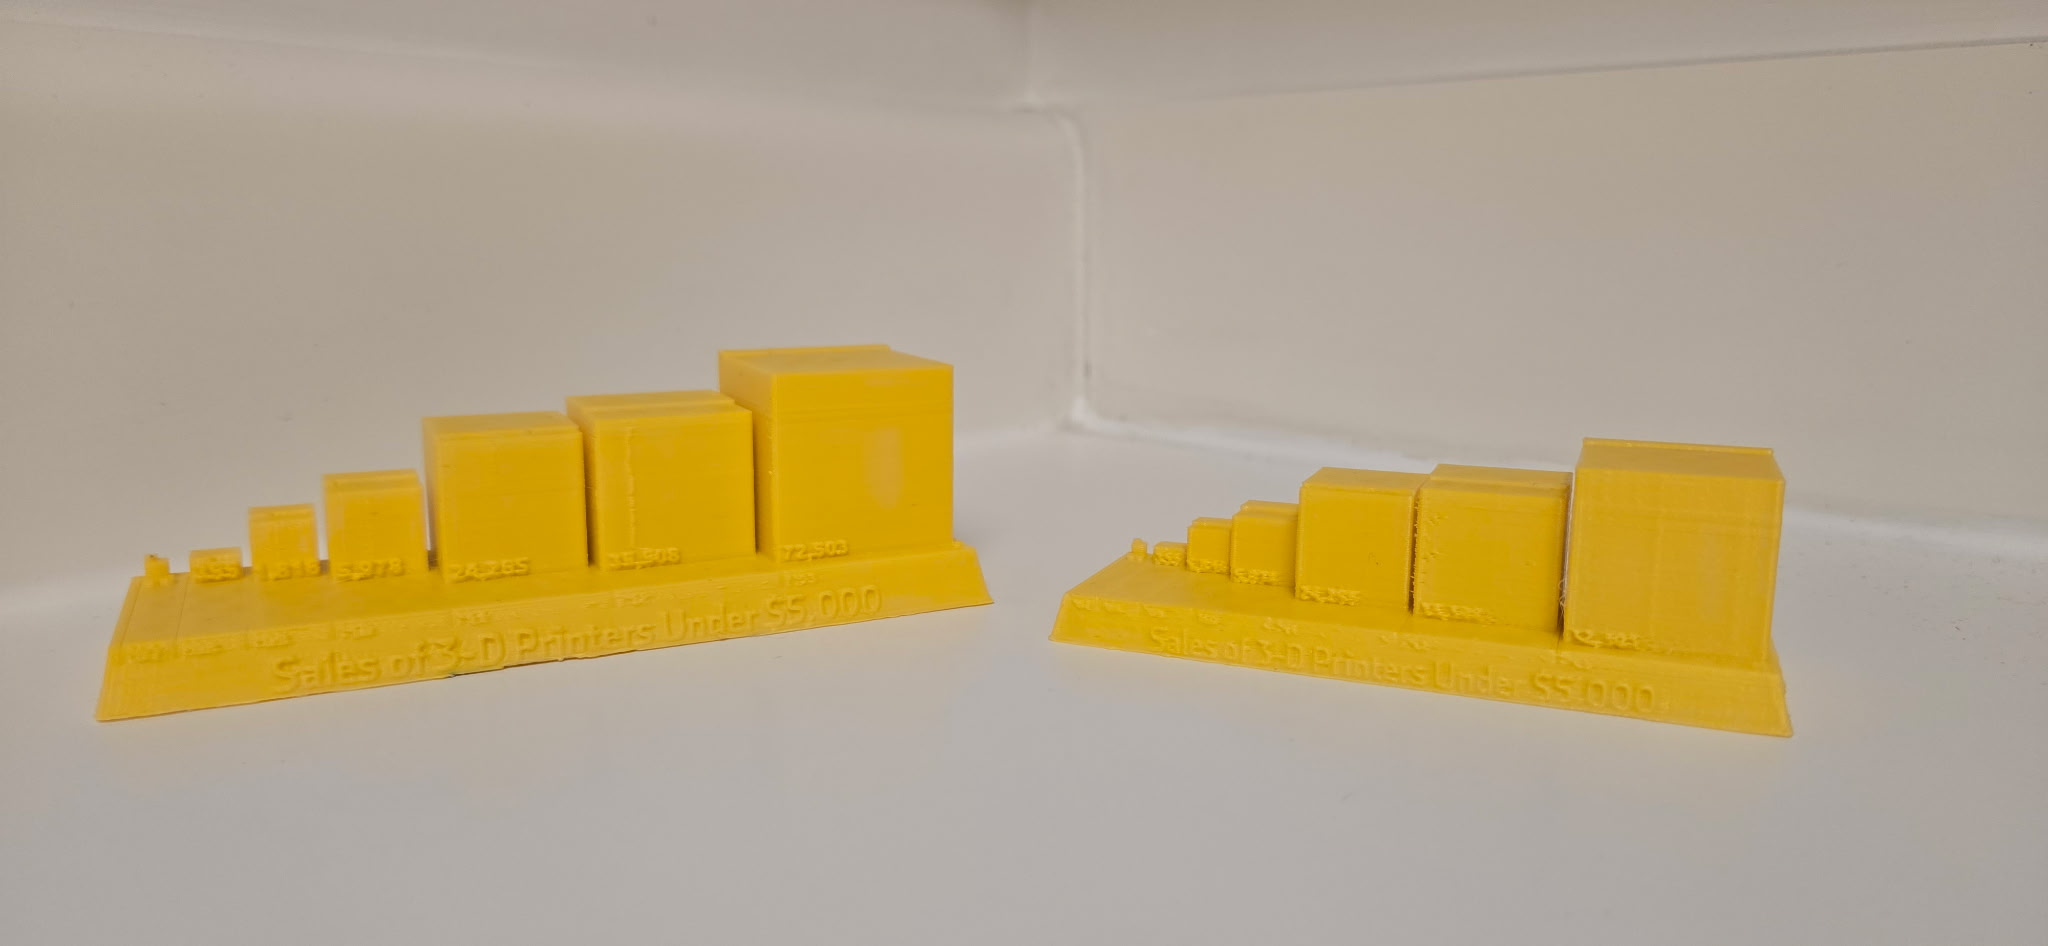
\includegraphics[width=\textwidth,height=2in]{images/wsj-myprint.jpg}

}

\subcaption[Replicated WSJ 3D print]{\label{fig-wsj-myprint}Replicated
print created in 2025}

\end{minipage}%

\caption{\label{fig-wsj}Figure~\ref{fig-wsj-orig} shows the original WSJ
print from 2014. Figure~\ref{fig-wsj-myprint} shows two prints created
with a Flash Forge Finder 3D Printer, where the smaller chart took 2
hours to print and the larger chart took 6 hours to print.}

\end{figure}%

\subsection{Creating 3D-Printed
Visualizations}\label{creating-3d-printed-visualizations}

The popularity of the 3D printer exploded in the early 2010s as the
technology became increasingly available and cheaper. This has led to
increased use of 3D printing in many focus areas, including healthcare
(Dodziuk, 2016) and engineering (V et al., 2023), but has seen only
limited use for statistical graphics. The creation of 3D-printed
statistical graphics involves generating an STL file and using it within
3D printing software to produce the final print file. This file can then
be transferred to a 3D printer, where the chart can be materialized.
Many software programs have the ability to create 3D statistical
graphics, but lack the ability to easily export the graphics into files
suitable for 3D printing.

Numerous software programs can create digital renderings of 3D charts.
Excel (Microsoft Corporation, 2025) has native support for creating
charts with 3D depth cues, but requires add-ins to produce charts using
3 axes. R (R Core Team, 2025) has several options for creating 3D charts
that have data on 3 axes (Morgan-Wall, 2024; e.g., Murdoch \& Adler,
2024; Sievert, 2020), but lacks support for creating depth charts. SAS
9.4 (\emph{SAS 9.4 ODS Graphics}, n.d.) has options such as PROC GCHART
for adding depth cues and PROC G3D for surface charts. Other popular
software programs contain similar capabilities, such as JavaScript
libraries, MATLAB, and Python.

While a number of tools exist for creating 3D data visualizations, the
pipeline of getting these charts into files compatible with 3D printing
is not widely automated. For example, R has some options using the
\texttt{rgl} (Murdoch \& Adler, 2024) and \texttt{rayshader}
(Morgan-Wall, 2024) packages, but both packages have limited tuning
parameters for their output files. Another option is to use 3D software,
such as OpenSCAD (Kintel, 2023), to manually create the charts, but
these software programs lack the ability to directly integrate
statistical information in the formulation of the charts. Without easy
tools for creating 3D print files from the original data source, the
process of created 3D-printed charts requires extensive manual effort to
create the print file.

Another consideration for 3D-printed charts is the inclusion of text
labels. These labels, and text annotations, are essential in
communicating the context of the data (Homestead, 2021). With
single-filament 3D printers, text can be incorporated in three primary
ways: (1) embossing, in which the text is raised above the surface of
the print; (2) engraving, in which the text is recessed into the
surface; or (3) applying external labels, such as stickers or ink.
Multi-filament 3D printers have the additional option to use a different
color for text labels, which can be applied to be either flush with the
surface of the chart or embossed for tangibility. However, Munzner
(n.d.) cautioned that the text of 3D charts may suffer from legibility
issues due to the distortion of the text when viewed at an angle. Few
recommendations exist for the incorporation of labels on data
physicalizations, but the use of labels should complement the
construction of the chart (Sauvé et al., 2022).

\section{Bar Charts in Research and
Practice}\label{bar-charts-in-research-and-practice}

One of the most common types of charts is the bar chart, characterized
by the use of rectangular geometries in a 2D space. Two variables are
mapped to the geometries of the bar chart, where one axis is dedicated
to a categorical variable of nominal or ordinal nature, and the other
axis is for a continuous variable to denote magnitude or a response.
These charts have been used over 200 years and remain a popular choice
for many modern data visualizations (Friendly \& Wainer, 2021). The use
of 3-dimensional elements in bar charts typically involve converting the
rectangular bars into rectangular prisms. Figure~\ref{fig-make-bar-3d}
shows an illustration of this transformation.

\begin{figure}

\begin{minipage}{0.50\linewidth}

\centering{


\includegraphics{images/make-bar-3d-1.png}

}

\subcaption[2D bar face]{\label{fig-bar3d-1}2D bar}

\end{minipage}%
%
\begin{minipage}{0.50\linewidth}

\centering{


\includegraphics{images/make-bar-3d-2.png}

}

\subcaption[Opposite bar face]{\label{fig-bar3d-2}Opposite face}

\end{minipage}%
\newline
\begin{minipage}{0.50\linewidth}

\centering{


\includegraphics{images/make-bar-3d-3.png}

}

\subcaption[Connecting bar faces]{\label{fig-bar3d-3}Connecting faces}

\end{minipage}%
%
\begin{minipage}{0.50\linewidth}

\centering{

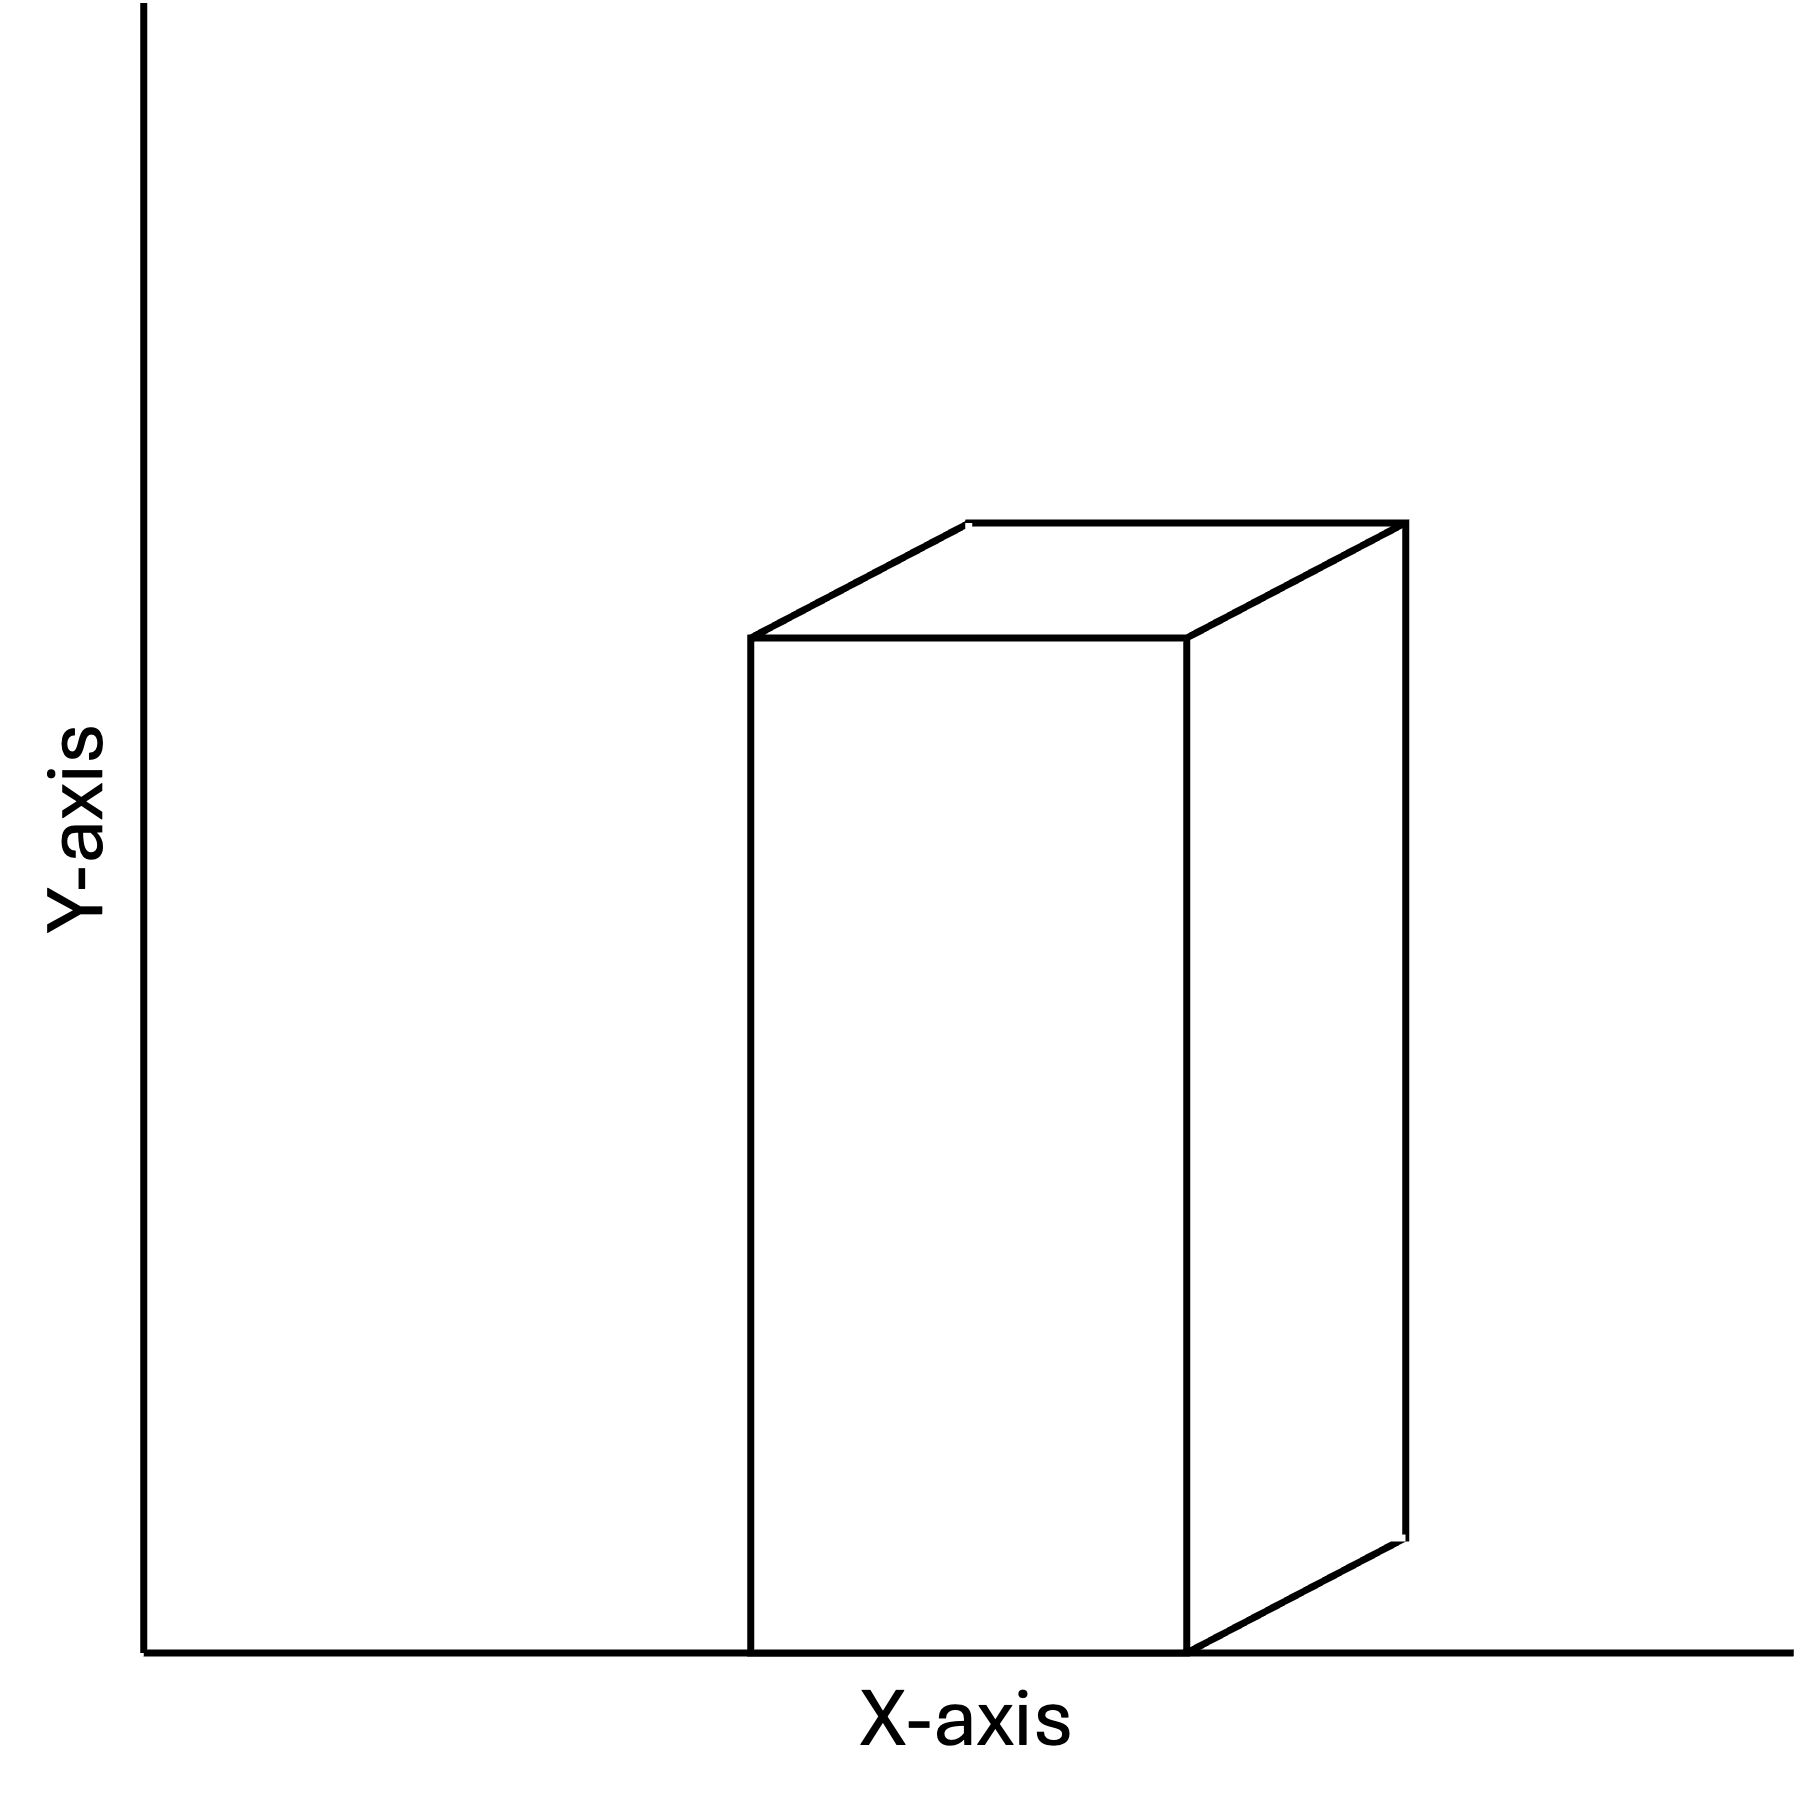
\includegraphics{images/make-bar-3d-4.png}

}

\subcaption[Solid 3D bar]{\label{fig-bar3d-4}Solid object}

\end{minipage}%

\caption{\label{fig-make-bar-3d}Construction of depth cues for a 2D bar
chart. In some cases, bar are constructed such that the y-axis
corresponds with the front face of the prism (as shown). Other 3D bar
charts may have the y-axis aligned with the back face.}

\end{figure}%

The naming convention for these types of bar charts is not consistent.
Many researchers in the visualization community call these 3D bar charts
due to the portrayal of three-dimensional space (Fischer, 2000; e.g.,
Zacks et al., 1998). Other times, the lack of information in the third
dimension results in the charts referred to as 2.5D charts (e.g.,
Tractinsky \& Meyer, 1999). To be consistent, we will refer to this
style as ``3D bar charts''.

\subsection{Against 3D Bar Charts}\label{against-3d-bar-charts}

Tufte (2001) called the use of 3D elements a ``fake perspective'' in his
description of ``chart junk'', which is where visual elements add
clutter to the data visualization. Other researchers (Stewart et al.,
2009; Zacks et al., 1998) have termed the perspective effect
``extraneous'' when referring to depth cues. The reasoning behind this
is fairly intuitive: why include additional noise when simpler
alternatives exist?

The seminal work of Cleveland \& McGill (1984) theorized that encoding
information in volumes would provide worse numerical estimation than for
encodings using positions, lengths, and areas. Their reasoning stems
from Stevens' Power Law (Stevens, 1957), a psychophysics formulation
that estimates a perceived stimulus magnitude \(p\) with the actual
magnitude \(a\) by \(p=ka^\alpha\). The estimation of \(\alpha\)
provides guidance as to which types of stimuli are most subject to
distortion from their true scale when \(\alpha=1\). Stevens (1957)
estimated \(\alpha\) to be approximately 1.1 for visual length and as
low as 0.9 for visual area. While the 3D bar charts do not lose their 2D
encodings, they do gain depth, and thus volume encodings. The effect of
volume versus area comparisons was noted earlier by Croxton \& Stein
(1932), where accuracy for ratio estimations was worse for cubes as
compared to bars and circles. When considering the dimensionality,
comparisons of lower dimensions tend to be less distorted to human
perception than higher dimensions.

From an artistic point of view, depth cues can obscure some elements of
the chart, resulting in a decrease in readability. For 3D bar charts,
this often occurs from the volumetric elements partially covering the
response axis. Consider Figure~\ref{fig-skewed} where the y-axis
corresponds to the back face of the rectangular prism. In this case, the
front and right faces do not directly correspond with the axis, thus
making it more difficult to extract values from the chart.

\begin{figure}

\centering{

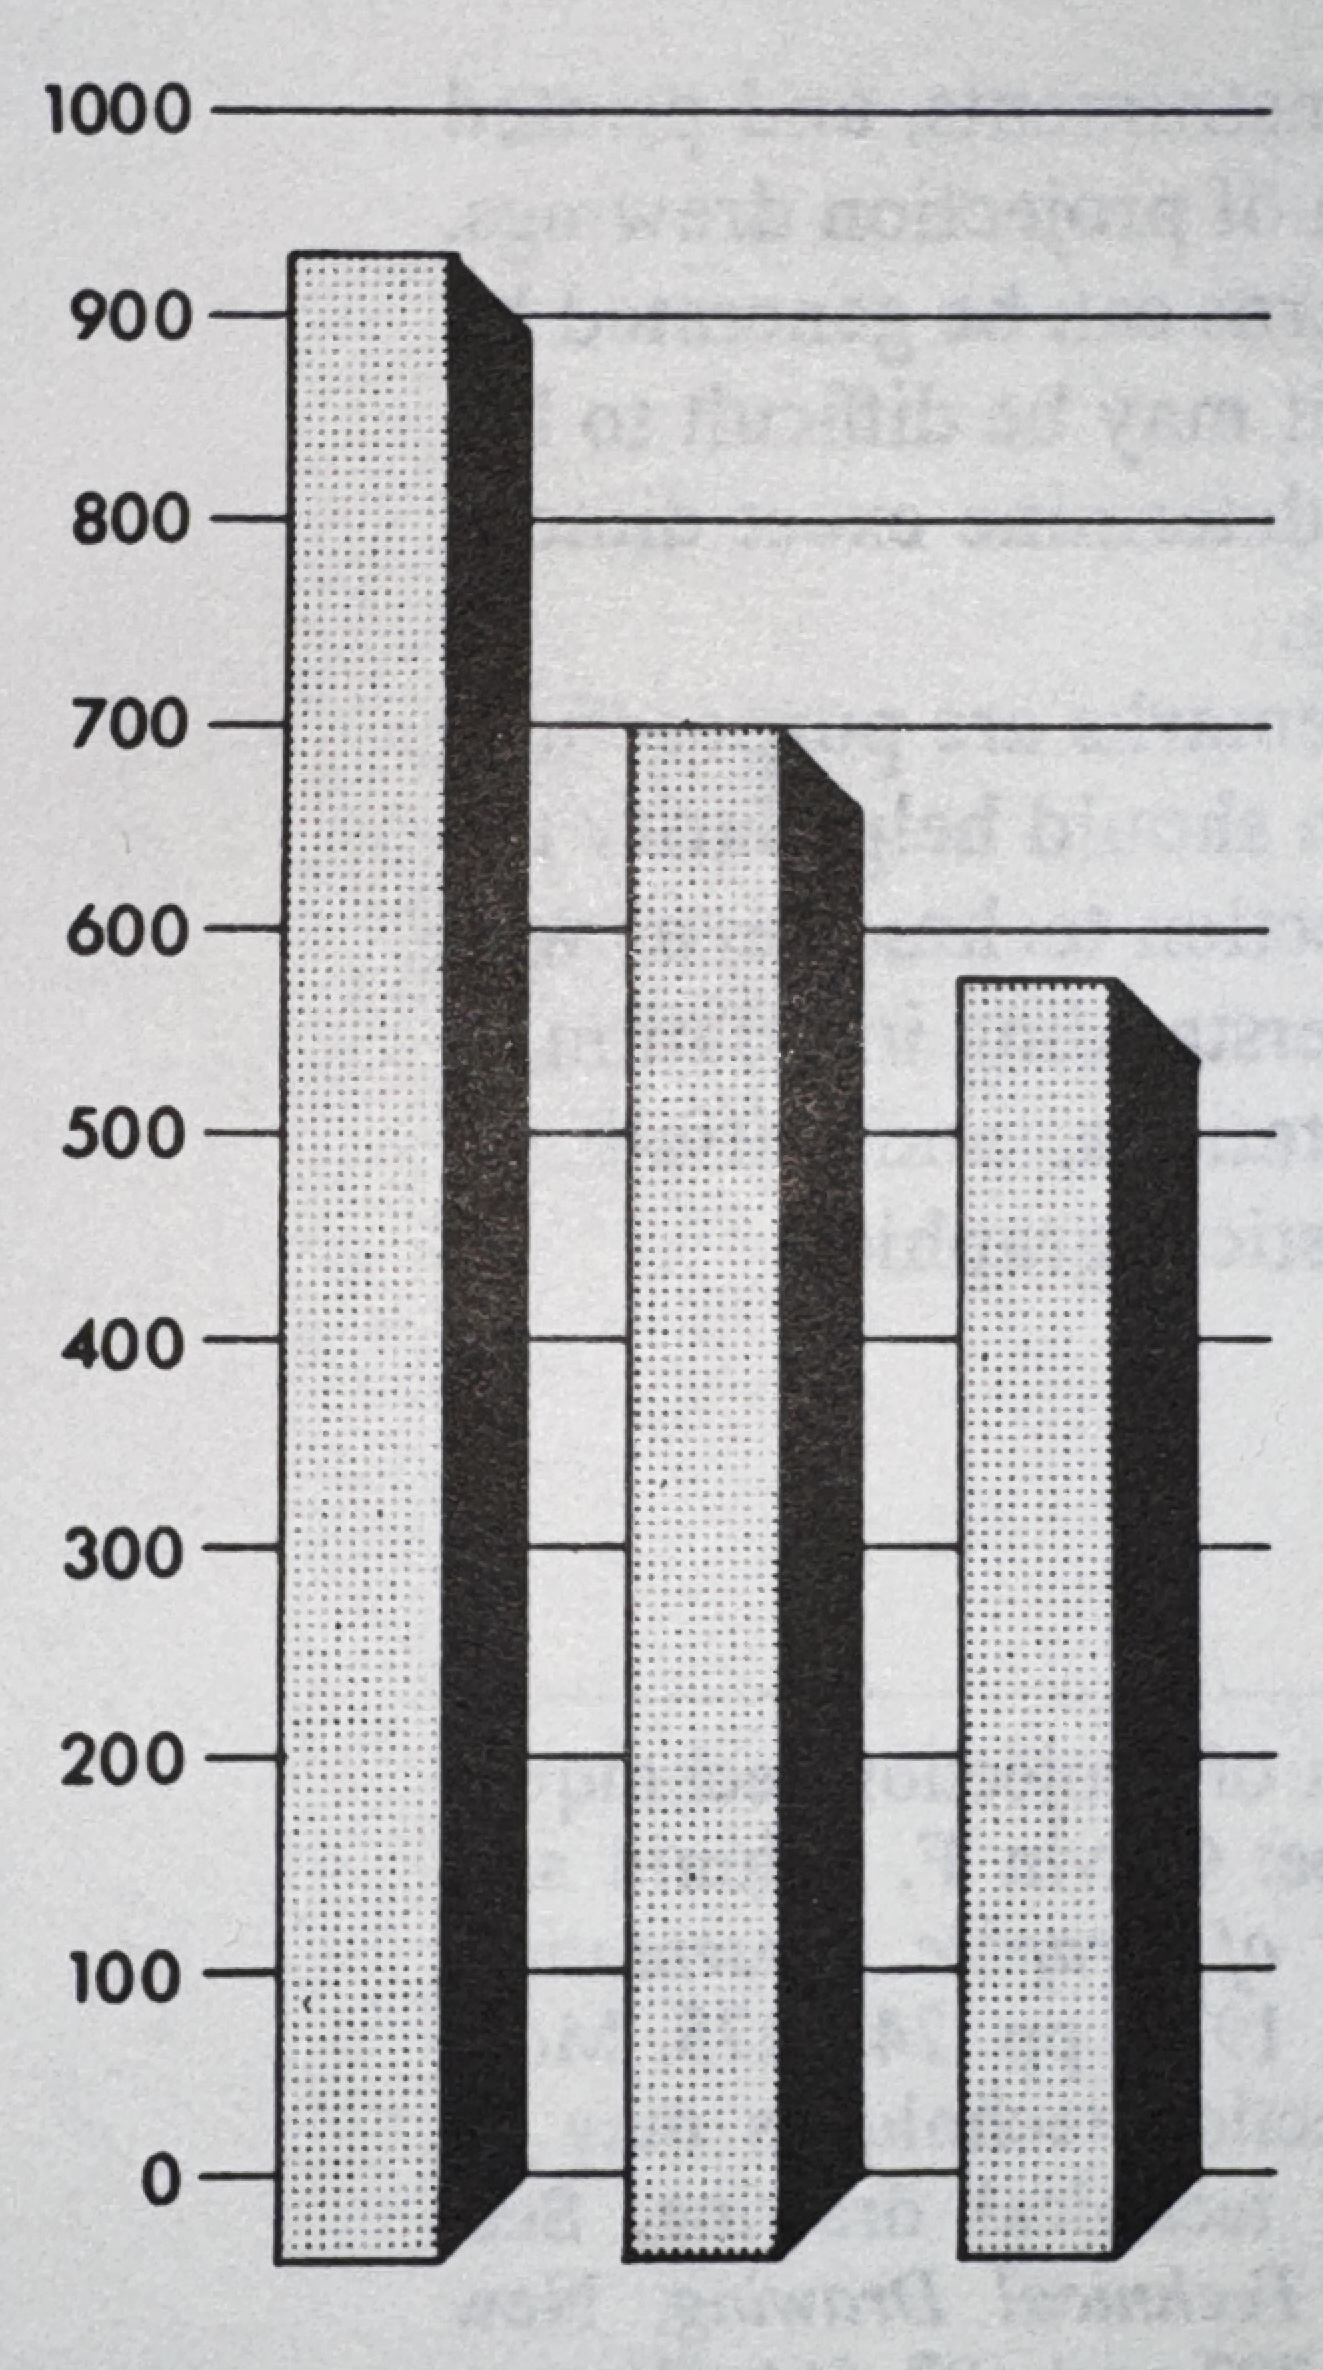
\includegraphics[width=3.35in,height=\textheight]{images/skewed-angle.jpg}

}

\caption[Skewed view overestimates bar heights]{\label{fig-skewed}Figure
from Schmid (1983) when discussing 3D visualizations. The viewing angle
for this chart would likely have viewers overestimate the values of the
bars by lining up the front face with the y-axis.}

\end{figure}%

\subsection{For 3D Bar Charts}\label{for-3d-bar-charts}

The primary motivations for using 3D bar charts are preference and
memorability. Levy et al. (1996) argued that depth cues can be useful in
these contexts. In three experiments involving over 100 psychology
students, participants were asked to select from a set of 2D and 3D
charts for different tasks. Their results suggested that students more
often preferred 3D charts when the goal was to enhance memory of the
chart, while preferences were about evenly split between 2D and 3D when
the task was to present information to others. Levy et al. (1996) also
suggested that the depth embellishments in 3D graphics may boost
memorability by making charts more visually distinctive.

The primary motivations for using 3D bar charts are preference and
memorability. Embellishments through the use of 3D elements could be
interpreted as more impressive, and thus better for the final polished
chart. If the chart is visually appealing, it may increase the
memorability by having those distinctive elements. A study of chart
tasks was conducted by Levy et al. (1996), where it was suggested that
3D charts are preferred for these reasons. Another study conducted by
Fisher et al. (1997) suggested similar preferences. In each of these
studies, 2D charts were preferred for extracting information, and
approximately half of participants preferred 3D charts for displaying
information. Levy et al. (1996) speculated that the preference for 3D
charts was to make the displays stand out to the viewer and thus more
memorable.

The idea of 3D charts increasing memorability aligns with broader
findings on ``chart junk,'' where non-data elements are suggested to aid
recall of information found in visualizations, though often at the cost
of longer processing times (Bateman et al., 2010; Borgo et al., 2012;
Peña et al., 2020). Similar increases in processing time have been
reported specifically for 3D bar charts (Fischer, 2000; Siegrist, 1996;
Stewart et al., 2009). The trade-off between information extraction and
memorability provides some evidence that 3D bar charts may have
context-specific roles in data visualizations.

The persistence of 3D bar charts reflects the influence of artistic
preferences in visualization. The added depth can make results appear
more striking, giving the impression of visual weight. Such
embellishments often appeal to audiences by enhancing visual impact,
even when they add little to the clarity of the data itself.

\subsection{Conflicting Empirical
Studies}\label{conflicting-empirical-studies}

Although Tufte (2001) argued against the use of 3D charts whenever
possible, empirical studies involving direct comparisons of 2D and 3D
bar charts have shown mixed results. In general, these studies focus on
metrics of accuracy and find that 3D bar charts tend to be either less
accurate or just as accurate as their 2D counterparts. Another common
metric is response time, where 3D charts tend to have longer response
times. Overall preference for one style of chart over another is a
subjective measurement, but has shown mixed results for the two styles
of charts.

\subsubsection{Accuracy}\label{accuracy}

Accuracy is a common metric in studies comparing 2D and 3D bar charts,
typically measured by either extracting a single numeric estimate or
making comparisons between two values. Here, the style of chart with
lower errors are considered to be the better chart. Many studies used
controlled environments for constructing stimuli, often displaying one
or two stimuli at a time, or controlling non-target stimuli. In
practice, charts are often more complex, displaying many stimuli without
drawing attention to particular values.

When only measuring accuracy, 3D bar charts tend to be less accurate
than their 2D counterparts (Stewart et al., 2009; Zacks et al., 1998).
However, this result is less prominent when introducing time delays
(Zacks et al., 1998, Experiment 2) or easier task complexity (Stewart et
al., 2009). Siegrist (1996) noted that bar positions and sizes also
affected performance accuracy, emphasizing that other factors contribute
to accuracy. It is also important to note that metrics of accuracy are
not conclusive, where sometimes there is no evidence of a difference
between 2D and 3D bar charts (Melody Carswell et al., 1991).

Of course, there are other less-studied factors that could affect
perceptual judgments of accuracy in 3D bar charts. In addition to
viewing parameters found in 2D bar chart studies (Fischer et al., 2005;
Rice et al., 2024), adding depth cues are also subject to viewing
angles, amount of depth, and field of view parameters. Viewing angle,
with respect to the axis, can mislead the reader into overestimating or
underestimating numerical quantities Figure~\ref{fig-skewed}. Zacks et
al. (1998) did not find a significant effect for the amount of
perception depth, but noted a trend such that increased exaggeration of
depth lowered their accuracy metric. Lastly, field of view is fixed for
the viewer, but can widely distort 3D renderings Figure~\ref{fig-fov}.
These factors add additional complexity, but are not widely studied for
the use of statistical graphics.

\begin{figure}

\begin{minipage}{0.33\linewidth}

\centering{

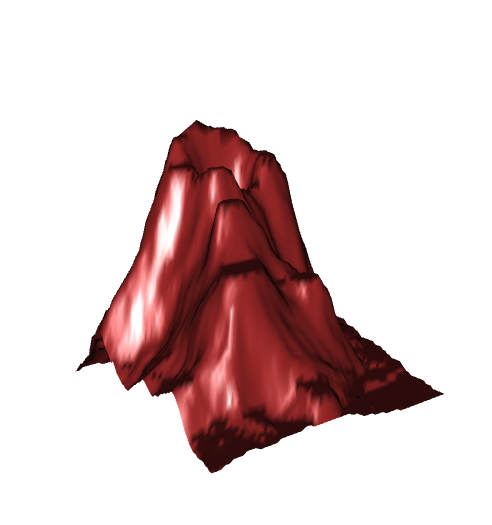
\includegraphics{images/fov-30.png}

}

\subcaption[FOV 30 degrees]{\label{fig-fov30}FOV: 30 degrees}

\end{minipage}%
%
\begin{minipage}{0.33\linewidth}

\centering{

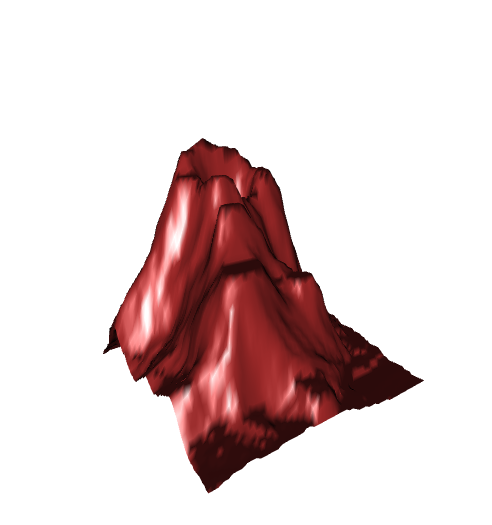
\includegraphics{images/fov-60.png}

}

\subcaption[FOV 60 degrees]{\label{fig-fov60}FOV: 60 degrees}

\end{minipage}%
%
\begin{minipage}{0.33\linewidth}

\centering{

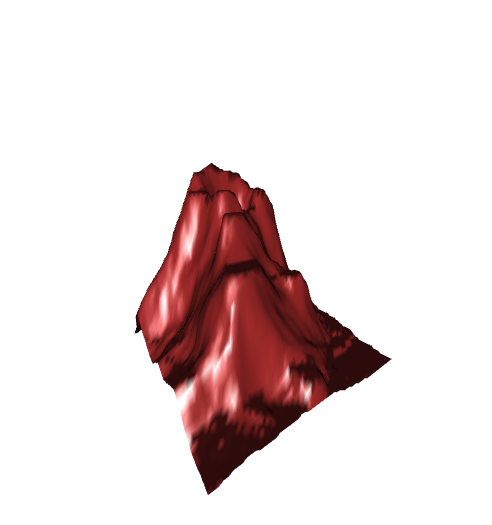
\includegraphics{images/fov-90.png}

}

\subcaption[FOV 90 degrees]{\label{fig-fov90}FOV: 90 degrees}

\end{minipage}%
\newline
\begin{minipage}{0.33\linewidth}

\centering{

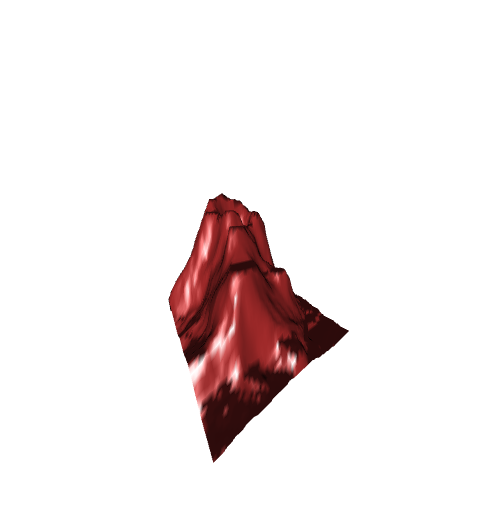
\includegraphics{images/fov-120.png}

}

\subcaption[FOV 120 degrees]{\label{fig-fov120}FOV: 120 degrees}

\end{minipage}%
%
\begin{minipage}{0.33\linewidth}

\centering{

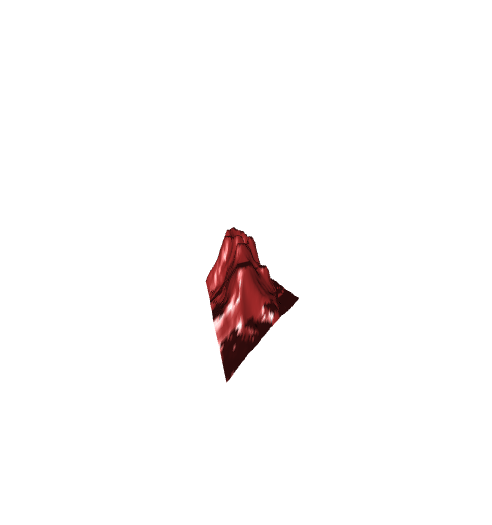
\includegraphics{images/fov-150.png}

}

\subcaption[FOV 150 degrees]{\label{fig-fov150}FOV: 150 degrees}

\end{minipage}%

\caption{\label{fig-fov}Multiple charts of the volcano dataset (R Core
Team, 2024) rendered using the \texttt{rgl} package (Murdoch \& Adler,
2024) in R. Each chart has a different field-of-view parameter, with the
amount of distortion increasing as the field-of-view (FOV) increases.}

\end{figure}%

\subsubsection{Response Times}\label{response-times}

The speed in making perceptual judgments is another common metric in
studies comparing types of charts. In theory, charts where questions can
be answered more quickly implies that the chart is better at
communicating information. However, response time is a poor metric in
situations of exploratory data analysis and long term interactions with
complex graphics (Vanderplas et al., 2020). When a question of interest
is known in advance, response time becomes a more viable metric.

Depth cues from 3D bar charts tend to increase the amount of time
required to answer questions (Fischer, 2000; Siegrist, 1996; Stewart et
al., 2009). Intuitively, additional complexity should require additional
time to process. For 3D bar charts, viewers need to align the response
axis with the rectangular prisms in order to determine the approximate
magnitude of the bar. Consider Figure~\ref{fig-skewed}, where the y-axis
denotes magnitude with respect to a hidden face of the bar. In order to
extract a numerical quantity, the viewer first has to align the axis
with the correct face of the prism before processing the magnitude. The
additional interaction of mentally aligning with the chosen viewing
parameters results in 3D charts needing additional time to process.

\subsubsection{Preference}\label{preference}

The debate between whether to use 2D or 3D graphics stems from a wider
adoption of 3D charts in practice. Computer graphics have made it easy
to produce charts of either dimensionality, resulting in creative
liberties for the creation of the chart for publication.
Figure~\ref{fig-ag-bar} showcases two examples of 3D bar charts from the
1978 Handbook of Agricultural Charts (\emph{1978 Handbook of
Agricultural Charts. Enlargements / {[}u.s. Department of
Agriculture{]}}, 1978) where other options exist for displaying the
data. Schmid (1983) (Chapter 8) also showcases many other 3D charts
published in official reports. Evidently, the persistence of 3D bar
charts has shown preferential use by maintaining a presence in many
software programs, including the widely used Microsoft Excel.

\begin{figure}

\begin{minipage}{0.50\linewidth}

\centering{

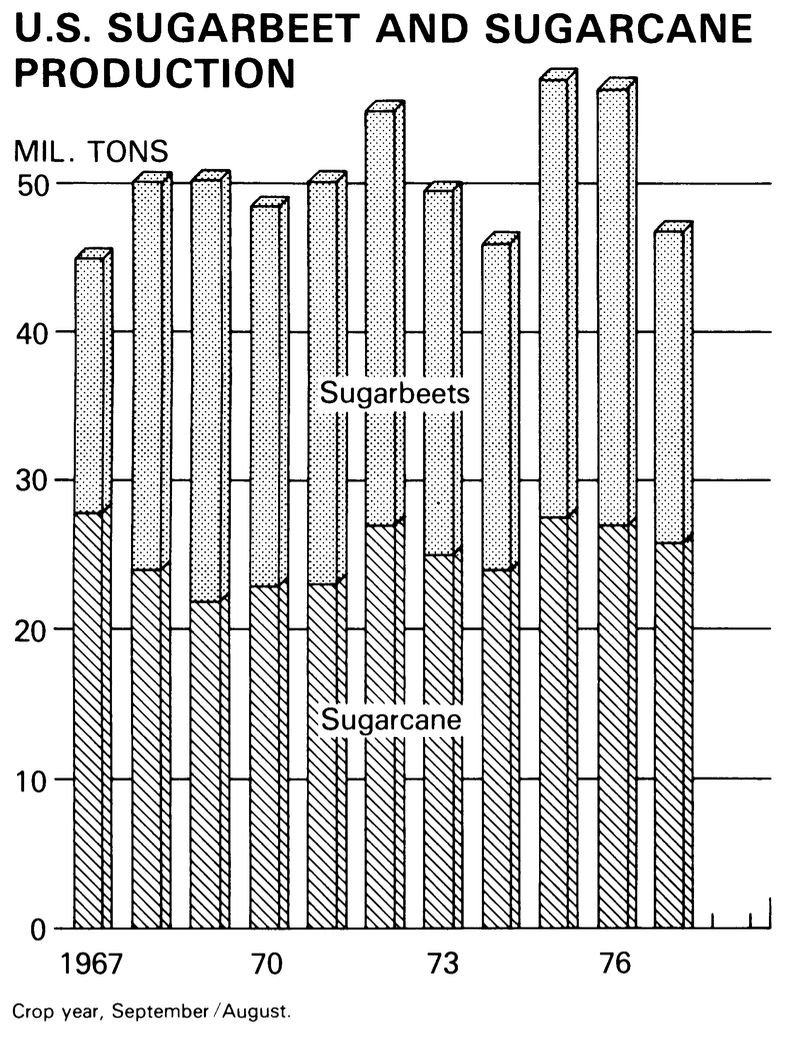
\includegraphics[width=\textwidth,height=2in]{images/preferance-example1.png}

}

\subcaption[Positive-value 3D bar chart]{\label{fig-ag-bar-pos}Bar chart
with strictly positive values}

\end{minipage}%
%
\begin{minipage}{0.50\linewidth}

\centering{

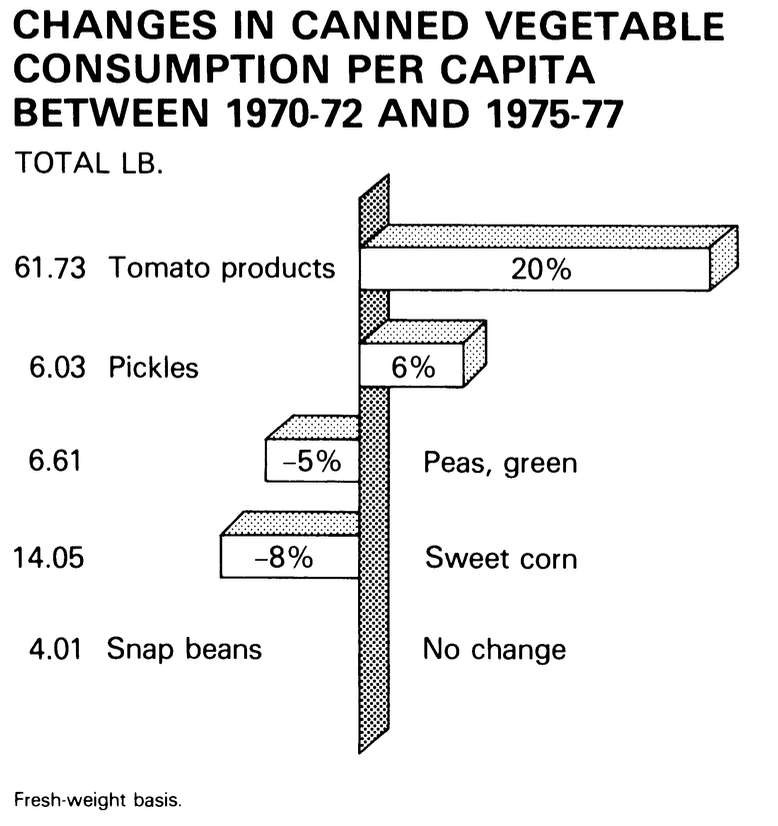
\includegraphics[width=\textwidth,height=2in]{images/preferance-example2.png}

}

\subcaption[Negative-value 3D bar chart]{\label{fig-ag-bar-neg}Bar chart
with negative values}

\end{minipage}%

\caption{\label{fig-ag-bar}Two examples of 3D bar charts found in
publication (\emph{1978 Handbook of Agricultural Charts. Enlargements /
{[}u.s. Department of Agriculture{]}}, 1978). This left image is a
stacked bar chart, using shadings to indicate sugarbeats and sugarcane.
The image on the right is a bar chart with positive and negative values
of changes in canned vegetable consumption.}

\end{figure}%

Preference for data visualizations can be categorized into visual appeal
and overall usefulness. Visual appeal is where perceptual tasks are not
a priority, and the goal is to have an image that is pleasant to the
viewer. Charts chosen for visual appeal may not accurately convey each
individual observation, but rather emphasize key trends of the data or
promote engagement with the visualization. Usefulness, on the other
hand, is a rating of how effective the viewer thought the chart was for
answering specific questions. This often comes in the form of comparing
multiple values, where accuracy in the comparisons is an essential
component of the chart. The purpose of the chart can be an influential
factor in deciding which chart type to use for displaying a dataset
(Levy et al., 1996).

When not tasked with estimating values, 3D bar charts tend to be more
visually appealing (Fisher et al., 1997; Levy et al., 1996; Stewart et
al., 2009). This may be in part due to the forced illusion of depth
which creates additional embellishments that would increase the
impression and memorability of the chart, as seen by other types of
Tufte's ``chart junk'' (Borgo et al., 2012; Peña et al., 2020). Despite
the visual appeal, 2D charts tend to be chosen for preference and ease
of use when making numerical estimations (Levy et al., 1996; Stewart et
al., 2009). The contrast between the visual appeal of 3D bar charts and
the utility of 2D bar charts is interesting to note since we would
intuitively expect charts that are easier to read as being the optimal
chart. This does not seem to be the case for the dimensionality of bar
charts.

\begin{figure}

\begin{minipage}{0.50\linewidth}
Three examples of chart preference.\end{minipage}%

\end{figure}%

\section{Heatmaps in Research and
Practice}\label{heatmaps-in-research-and-practice}

When creating charts for three or more variables, it becomes
increasingly complex to visualize data (Grinstein \& Trutschl, 2001).
One option is to map the additional variables to aesthetics using
gestalt principles (Vanderplas et al., 2020), which includes making use
of color, size, and/or shapes to denote information. However, not every
aesthetic is compatible with every type of variable. Color can be used
to map either continuous variables with gradient scales or categorical
variables with palettes. Size is typically reserved for continuous
variables, where larger values correspond to a larger quantity. Shapes
tend to have finite distinguishable representations in order to
represent categorical variables. Examples of good and poor cases for
each of these aesthetics are presented in Figure~\ref{fig-gestalt}.

\begin{figure}

\begin{minipage}{0.50\linewidth}

\centering{

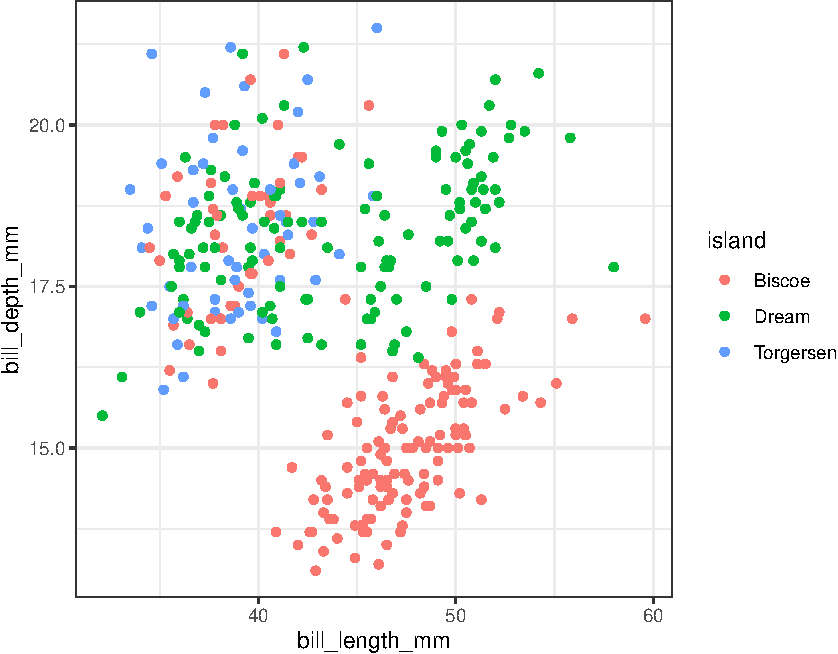
\includegraphics[width=0.9\textwidth,height=0.9\textheight]{index_files/figure-pdf/fig-gestalt-1.pdf}

}

\subcaption[Gestalt channels in penguin
scatterplots]{\label{fig-gestalt-1}Color mapped to categorical
variable.}

\end{minipage}%
%
\begin{minipage}{0.50\linewidth}

\centering{

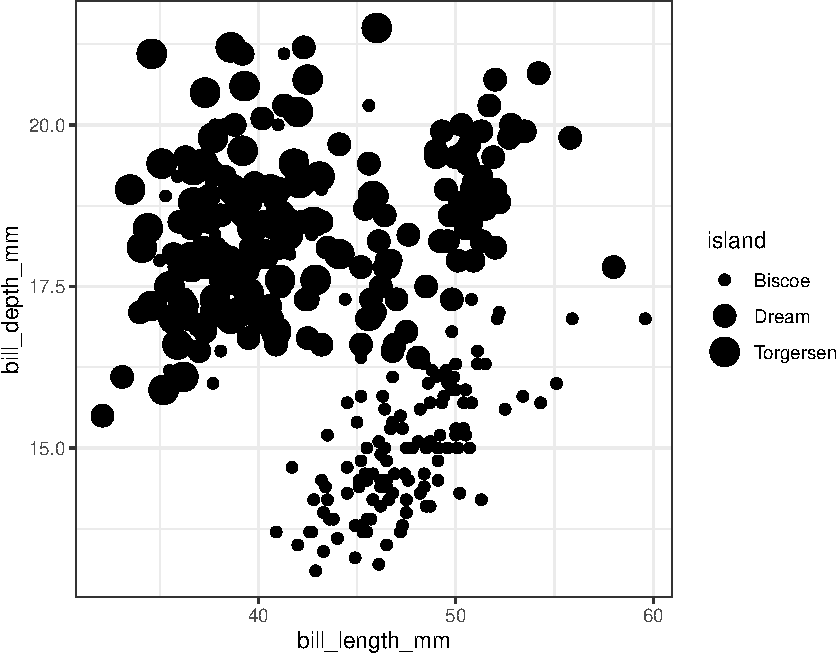
\includegraphics[width=0.9\textwidth,height=0.9\textheight]{index_files/figure-pdf/fig-gestalt-2.pdf}

}

\subcaption[Gestalt channels in penguin
scatterplots]{\label{fig-gestalt-2}Size mapped to categorical variable.}

\end{minipage}%
\newline
\begin{minipage}{0.50\linewidth}

\centering{

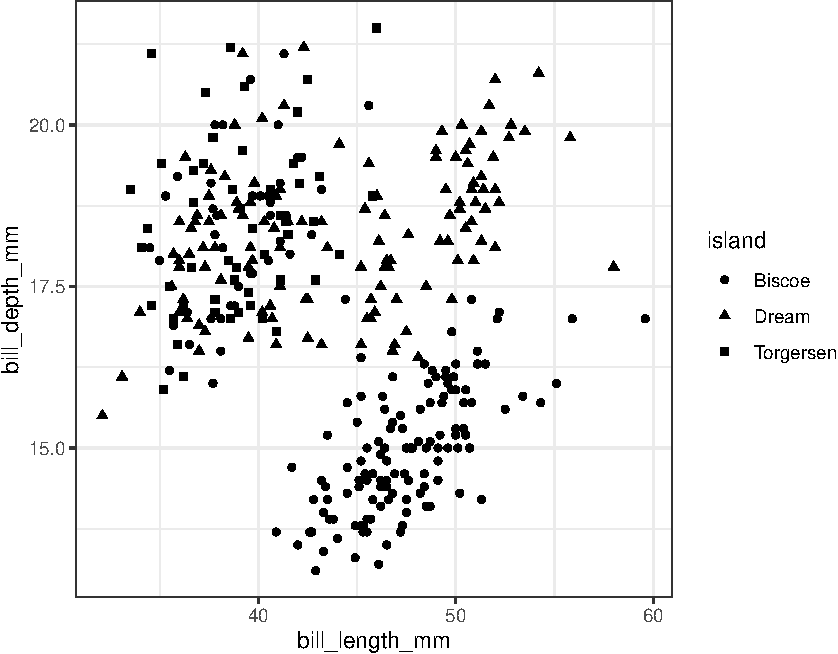
\includegraphics[width=0.9\textwidth,height=0.9\textheight]{index_files/figure-pdf/fig-gestalt-3.pdf}

}

\subcaption[Gestalt channels in penguin
scatterplots]{\label{fig-gestalt-3}Shape mapped to categorical
variable.}

\end{minipage}%
%
\begin{minipage}{0.50\linewidth}

\centering{

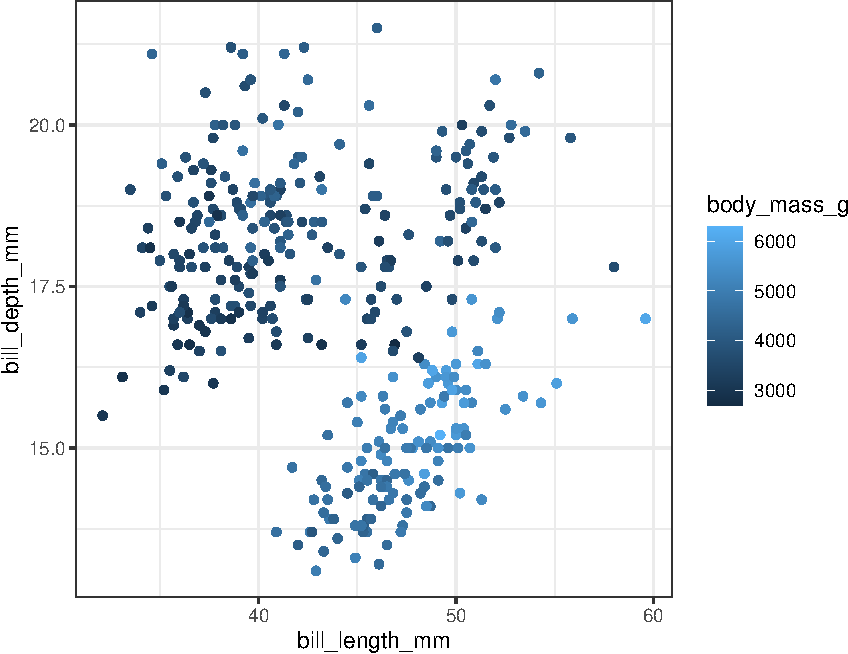
\includegraphics[width=0.9\textwidth,height=0.9\textheight]{index_files/figure-pdf/fig-gestalt-4.pdf}

}

\subcaption[Gestalt channels in penguin
scatterplots]{\label{fig-gestalt-4}Color mapped to continuous variable.}

\end{minipage}%
\newline
\begin{minipage}{0.50\linewidth}

\centering{

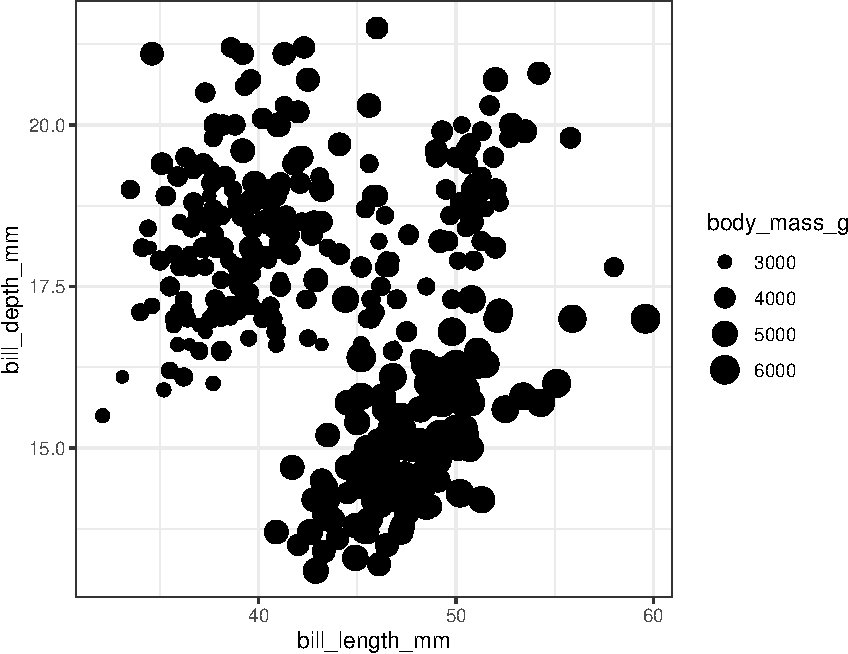
\includegraphics[width=0.9\textwidth,height=0.9\textheight]{index_files/figure-pdf/fig-gestalt-5.pdf}

}

\subcaption[Gestalt channels in penguin
scatterplots]{\label{fig-gestalt-5}Size mapped to continuous variable.}

\end{minipage}%
%
\begin{minipage}{0.50\linewidth}

\centering{

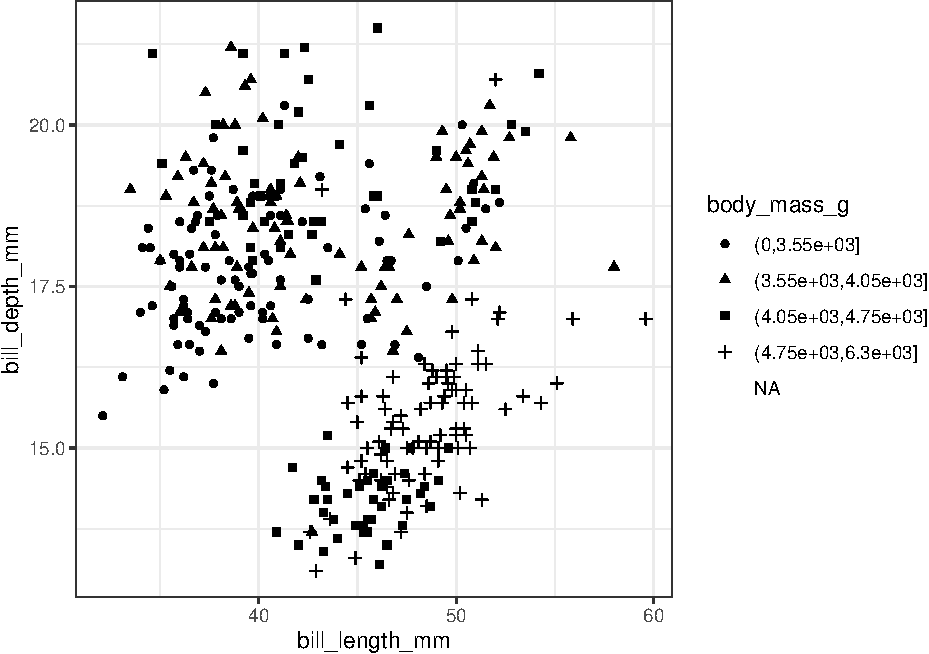
\includegraphics[width=0.9\textwidth,height=0.9\textheight]{index_files/figure-pdf/fig-gestalt-6.pdf}

}

\subcaption[Gestalt channels in penguin
scatterplots]{\label{fig-gestalt-6}Shape mapped to continuous variable.}

\end{minipage}%

\caption{\label{fig-gestalt}Examples of color, size, and shape for
scatterplots of the penguins dataset (Horst et al., 2020).}

\end{figure}%

Heatmaps are a type of chart that can be used with two nominal or
ordinal variables, and a continuous response variable. In
two-dimensional formats, gradient fills are often used to denote the
magnitude of the responses, utilizing a gradient scale. When represented
in three dimensions, height is the primary mapping of the response of
the heatmap. Due to the height aesthetic, 3D heatmaps are sometimes
referred to as ``height maps'', particularly when spatial coordinates
are involved. Since the color and/or height of the response variable can
only be mapped once to each combination of x and y coordinates, heatmaps
are generally used to summarize responses, such as averages or
single-point observations. This makes heatmaps especially useful for
visualizing patterns and trends across large datasets in a compact and
interpretable format.

\begin{figure}

\begin{minipage}{0.50\linewidth}

\centering{

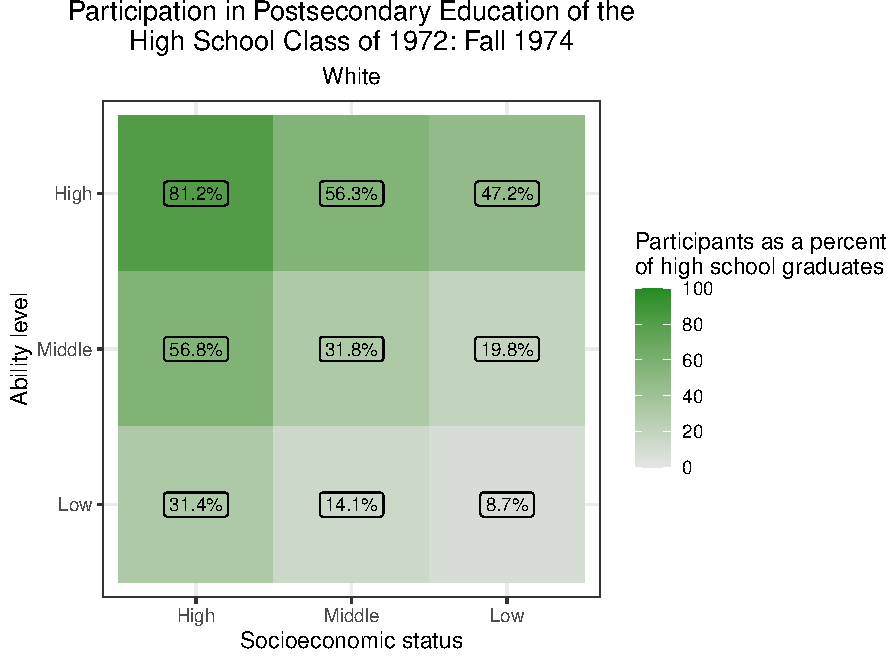
\includegraphics{index_files/figure-pdf/fig-heatmap2d-1.pdf}

}

\subcaption[2D color versus 3D height heatmap
encoding]{\label{fig-heatmap2d-1}2D heatmap}

\end{minipage}%
%
\begin{minipage}{0.50\linewidth}

\centering{

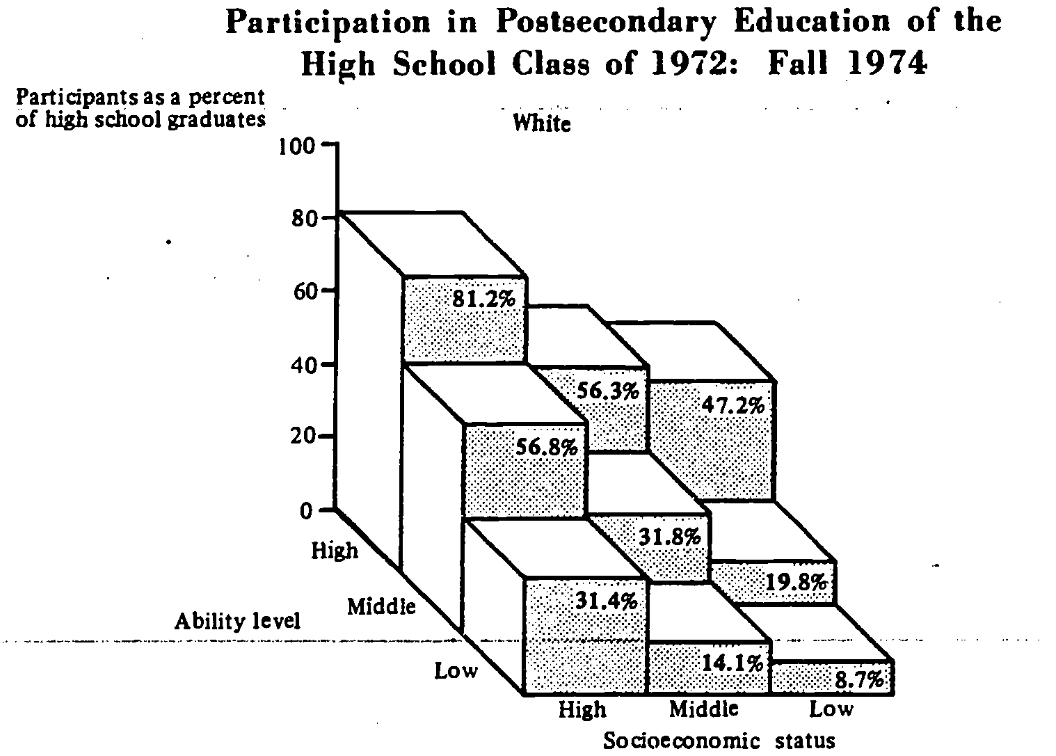
\includegraphics[width=3.52in,height=\textheight]{images/heatmap3d.png}

}

\subcaption[2D color versus 3D height heatmap
encoding]{\label{fig-heatmap2d-2}3D heatmap}

\end{minipage}%

\caption{\label{fig-heatmap2d}Heatmaps created with data from for
Educational Statistics et al. (1977). The 2D heatmap represents the
percentage of high school graduates participating in postsecondary
education using a gradient color scale, whereas the 3D heatmap uses
height. In each chart, there is an increasing association with
postsecondary education with ability level and socioeconomical status.}

\end{figure}%

\subsection{Empirical Studies of 2D and 3D
Heatmaps}\label{empirical-studies-of-2d-and-3d-heatmaps}

Unlike 2D and 3D bar charts, the dimensional comparison for heatmaps has
not been widely studied. This may be attributed to the complex designs
of heatmaps, where there are many possible variables to consider. For
example, the complex nature of color scales having an influential role
in the perception of 2D heatmaps (Breslow et al., 2009; Liu \& Heer,
2018a; Reda \& Papka, 2019). It has also been observed that neighboring
values may influence the ability to extract values, either by
distraction or visual illusions {[}zacks1998; VanderPlas \& Hofmann
(2015){]}. The dimensionality of heatmaps requires the additional
consideration of mapping color scales into heights, which is a process
that has no literal translation. Depending on the scaling when mapping
color to height, features may become overly smoothed or overly
exaggerated. An example of this mapping discrepancy is shown in
Figure~\ref{fig-color-height}. We expect that these numerous design
choices contribute to the lack of research on 2D and 3D heatmaps.

\begin{figure}

\begin{minipage}{0.50\linewidth}

\centering{

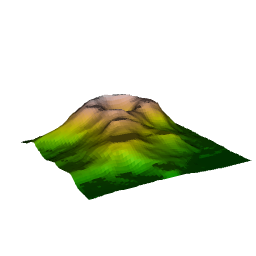
\includegraphics{images/height-color-0.3.png}

}

\subcaption[Compressed height scale]{\label{fig-flat3d}Flatter height
scale}

\end{minipage}%
%
\begin{minipage}{0.50\linewidth}

\centering{

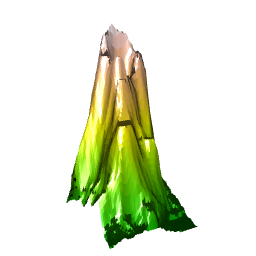
\includegraphics{images/height-color-2.png}

}

\subcaption[Expanded height scale]{\label{fig-tall3d}Stretched height
scale}

\end{minipage}%

\caption{\label{fig-color-height}Two figures representing the volcano
dataset (R Core Team, 2024) using different height scaling factors. Both
figures use the same color scale, but there is no ``correct''
translation of color into the measurable height.}

\end{figure}%

In 2D heatmaps, the choice of color palettes can influence the
perception of numerical estimations (Liu \& Heer, 2018b; Molina Lopez et
al., 2023; Zhang et al., 2023). Some gradient scales are easier to
extract values from than others, and other gradient scales are better at
displaying contrasts between values. Additionally, the use of colors
requires accessibility considerations for people with color
deficiencies. The relationship between color and 2D heatmaps possibly
contributes to the difficulties of direct translations of 2D heatmaps
into 3D heatmaps.

\begin{figure}

\begin{minipage}{0.25\linewidth}

\centering{


\includegraphics{index_files/figure-pdf/fig-colorblind-1.pdf}

}

\subcaption[Inferno palette under color-vision
deficiencies]{\label{fig-colorblind-1}Original palette}

\end{minipage}%
%
\begin{minipage}{0.25\linewidth}

\centering{


\includegraphics{index_files/figure-pdf/fig-colorblind-2.pdf}

}

\subcaption[Inferno palette under color-vision
deficiencies]{\label{fig-colorblind-2}Deutan (red-green)}

\end{minipage}%
%
\begin{minipage}{0.25\linewidth}

\centering{


\includegraphics{index_files/figure-pdf/fig-colorblind-3.pdf}

}

\subcaption[Inferno palette under color-vision
deficiencies]{\label{fig-colorblind-3}Protan (red-green)}

\end{minipage}%
%
\begin{minipage}{0.25\linewidth}

\centering{


\includegraphics{index_files/figure-pdf/fig-colorblind-4.pdf}

}

\subcaption[Inferno palette under color-vision
deficiencies]{\label{fig-colorblind-4}Tritan (blue-yellow)}

\end{minipage}%

\caption{\label{fig-colorblind}Effect of color deficiencies on the
inferno palette from (\textbf{viridis?}).}

\end{figure}%

Only a few studies have directly compared the dimensionality of
statistical graphics (Jeong et al., 2025; Kraus et al., 2020). Conducted
primarily in virtual reality, these studies suggest that 2D and 3D
charts each offer advantages depending on the task. Two-dimensional
charts generally produced higher interpretation accuracy and better
recognition of overall distributional patterns. In contrast,
three-dimensional charts were more effective for estimating single
values and supporting long-term recall. Taken together, these findings
highlight dimensionality as an important consideration when selecting
visual displays for specific analytic goals.

\section{State of Data Physicalization in 3D Statistical
Graphics}\label{state-of-data-physicalization-in-3d-statistical-graphics}

While numerous studies explored the dimensionality of statistical
graphics in 2D renderings, only a few studies empirically evaluated
their effectiveness in 3D environments. Jansen et al. (2013) conducted
one of the first studies with physical 3D heatmaps and focused on task
completion times for estimations, suggesting that physical 3D heatmaps
were better for extracting information. Jansen et al. (2013) also
measured errors in estimations, but did not detect differences
attributed to chart types. A series of experiments by Simon Stusak
evaluated the memorability of digital and physical bar charts, which
suggested that physical 3D bar charts may improve the ability to recall
information (Stusak et al., 2015; Stusak et al., 2016). To date,
physical statistical graphics is a niche area in data visualizations and
is largely unexplored.

\section{Methods for Evaluating Visualization
Effectiveness}\label{methods-for-evaluating-visualization-effectiveness}

\subsection{What makes a good chart?}\label{what-makes-a-good-chart}

There are many aspects for designing good data visualizations.
Vanderplas et al. (2020) discussed various approaches to testing
graphics, including numerical estimations, speed, and error rates. These
metrics are fairly common to measure when comparing 2D and 3D charts
(Cleveland \& McGill, 1984; Croxton \& Stein, 1932; Hughes, n.d.), but
they do not represent the full picture of what makes one type of chart
better than another. As observed by Levy et al. (1996), the objectives
of the chart can determine which type of chart should be used. While
many metrics exist, the practical limitation of testing generally allows
for only a few metrics to be tested at a given time.

Many studies involving statistical graphics tend to rely on numerical
estimations for recommending data visualization practices. This is
particularly useful given the role that data visualizations play in the
understanding of underlying datasets, which is to understand data
structures and relationships (Tukey, 1965). Successful visualizations
should be able to translate tables into figures that rapidly convey
values and patterns found within the data structures. In this research,
we focus primarily on numerical estimations while also recording task
completion times.

\subsection{Designing studies for numerical
estimations}\label{designing-studies-for-numerical-estimations}

Many studies in graphical perception follow the same general format as
Cleveland \& McGill (1984). Their work has been credited with over 2,500
citations, which indicates the importance of testing features of
statistical graphics. Since 1984, the methods of analyzing and
conducting studies on statistical graphics have evolved alongside
statistical methods and technological progress (e.g., Hofmann et al.,
2012; Vanderplas et al., 2020), but the structure of experimental
designs involving numerical estimations tends to remain similar. Tasks
typically involve the comparison of two stimuli, where the question is
``how much bigger/smaller is one value compared to the other?'' The
phrasing of this question needs careful consideration since mental
subtractive processes are perceived differently from mental ratio
processes (Hagerty \& Birnbaum, 1978; Veit, n.d.). Our work, like many
others in the InfoViz community, follow a procedure similar to Cleveland
\& McGill (1984).

Cleveland \& McGill (1984) asked participants two questions when making
comparisons between two values on a chart: which of the two values was
the smaller, and what percentage the smaller was of the larger. The
first question clarified if the participants were looking at the values
correctly for the second question, and the second question is an
estimation of \(A/B\), where \(A<B\). Accuracy was measured by
\(\log_2(|\text{True value}-\text{Estimated value}|+1/8)\), using the
trimmed averages when bootstrapping confidence intervals. This measure
of error was used to assess which type of chart was better and provided
recommendations for how to display information. A replication performed
by Heer \& Bostock (2010) used Amazon's Mechanical Turk, which also
found similar recommended chart features using a crowdsourcing platform.
Many other studies tend to use similar types of questions when tasking
participants to make numerical estimations.

When designing studies for numerical estimation, the choice of \(A/B\)
is an important consideration. Many researchers seemingly choose ratios
in an arbitrary fashion or follow previously established work (e.g.,
Zacks et al. (1998) used the same ratios as Melody Carswell et al.
(1991)). Examples of ratios used in several studies are provided in
Figure~\ref{fig-ratios}. However, the magnitude of stimuli and ratios
are suggested to be a contributing factor to the amount of error in
estimations (Cleveland \& McGill, 1984; Zacks et al., 1998).
Additionally, participants may display an anchoring effect if the values
are close to certain increments (e.g., estimating 55\% as 50\%). This
suggests that the selection of ratios for estimation should cover a wide
range of possible ratios.

Several calculations for error can be considered when estimating
accuracy. The magnitude of error is calculated as
\(|\text{Guess}-\text{True value}|\), which is how far away a
participant's estimate is from the target value. Removing the absolute
value gives directional error, which allows for estimates to indicate
bias of overestimation or underestimation. Since ratio estimations tend
to be exponential (Veit, n.d.), it is also common to use the logarithmic
transformation, \(\log|\text{Error}|\), to address non-normality for the
magnitude of error. When reporting which chart type is more accurate in
the extraction of information, the calculation of error needs to be
clearly defined.

The type of estimation task can influence how participants respond with
their estimates. Psychophysics has demonstrated that asking participants
to estimate ratios elicits a different mental process than when asking
participants to estimate differences (Birnbaum \& Mellers, 1978; Veit,
n.d.). Estimations of ratios tend to fall on an exponential scale, where
larger differences in stimuli result in smaller differences of estimated
ratios. This makes \(\log|\text{Error}|\) a natural choice for measuring
ratio estimation tasks, similar to how Cleveland \& McGill (1984)
measured error. Measurements of differences tend to be estimated
linearly, where estimated differences are the same regardless of
differences in stimuli. Modern statistical methodology is able to
accommodate these linear and exponential relationships, as long as the
estimation task is consistent for each trial.

\begin{figure}

\begin{minipage}{0.50\linewidth}

\centering{

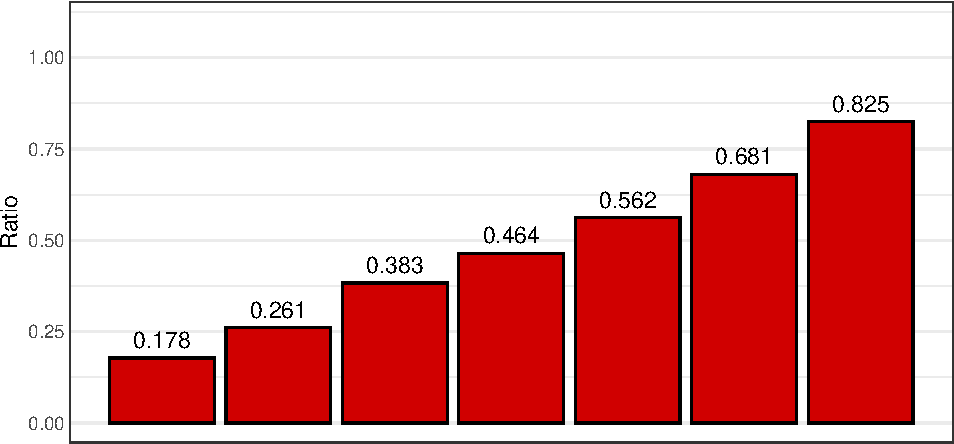
\includegraphics[width=0.9\textwidth,height=0.9\textheight]{index_files/figure-pdf/fig-ratios-1.pdf}

}

\subcaption[Ratios in prior graphical perception
studies]{\label{fig-ratios-1}Cleveland \& McGill (1984)}

\end{minipage}%
%
\begin{minipage}{0.50\linewidth}

\centering{

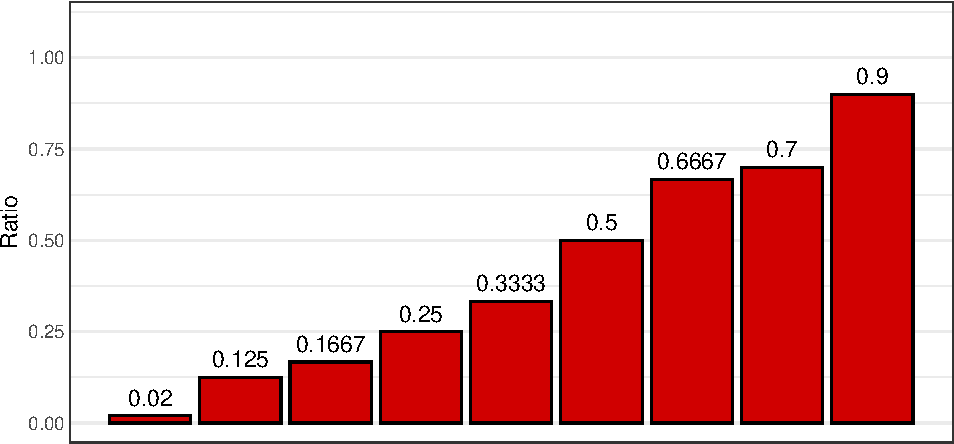
\includegraphics[width=0.9\textwidth,height=0.9\textheight]{index_files/figure-pdf/fig-ratios-2.pdf}

}

\subcaption[Ratios in prior graphical perception
studies]{\label{fig-ratios-2}Croxton \& Stein (1932)}

\end{minipage}%
\newline
\begin{minipage}{0.50\linewidth}

\centering{

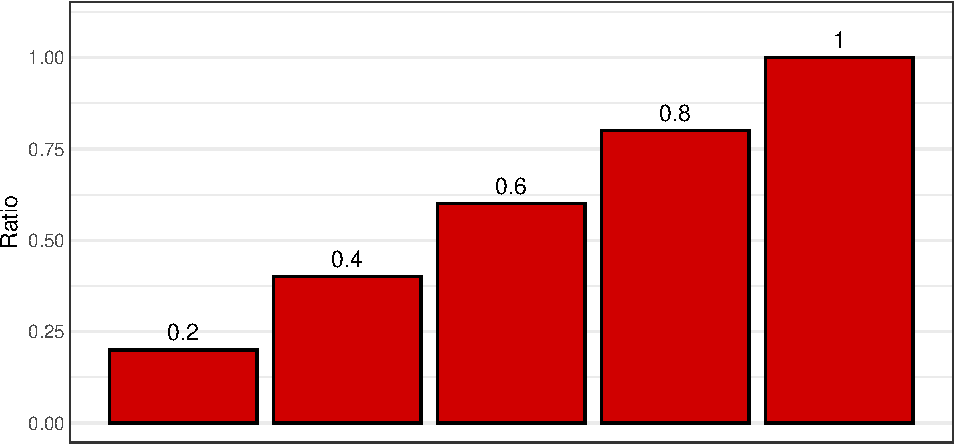
\includegraphics[width=0.9\textwidth,height=0.9\textheight]{index_files/figure-pdf/fig-ratios-3.pdf}

}

\subcaption[Ratios in prior graphical perception
studies]{\label{fig-ratios-3}Zacks et al. (1998), Experiment 1}

\end{minipage}%
%
\begin{minipage}{0.50\linewidth}

\centering{

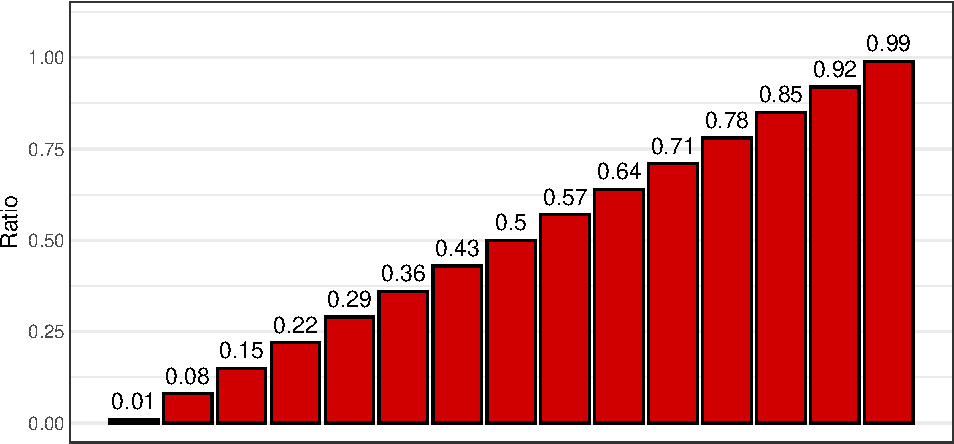
\includegraphics[width=0.9\textwidth,height=0.9\textheight]{index_files/figure-pdf/fig-ratios-4.pdf}

}

\subcaption[Ratios in prior graphical perception
studies]{\label{fig-ratios-4}Zacks et al. (1998), Experiment 3}

\end{minipage}%

\caption{\label{fig-ratios}Ratios used by several studies}

\end{figure}%

\section{Research Gaps and Study
Motivation}\label{research-gaps-and-study-motivation}

It is generally advised to avoid using 3D data visualizations whenever
possible, although previous studies often contradict this statement
through mixed findings. The main contributing factor tends to be the
role of the third dimension. When the third dimension is used for depth,
2D charts are generally preferred for better numerical extractions and
quicker completion times. On the contrary, using the third dimension for
displaying information can provide better estimates than 2D
alternatives. In addition, 3D charts tend to be chosen for their ability
to improve, or attempt to improve, the memorability of the data. This
makes previous research inconclusive on a superior chart dimensionality.

Despite extensive study of graphical dimensionality, these findings are
almost exclusively based on 2D projections presented on paper or digital
displays. As a result, current recommendations may not generalize to
contexts in which the third dimension is physically realized rather than
visually implied. Physical charts allow for natural interactions and
promote additional engagement with the data structures. However, current
literature provides little guidance on the construction or effectiveness
of physical charts.

In this research, we explore the the physical dimensionality of 2D and
3D statistical graphics. In Chapter 1, we explore the dimensionality of
bar charts using a pilot study that partially replicates the work of
Cleveland \& McGill (1984). We then expand the study in Chapter 2 as an
experiential learning project for an undergraduate introductory
statistics course and collect information on how students reflected on
various parts of the scientific process. Chapter 3 takes the ideas of
Chapter 1 and Chapter 2 and replaces bar charts with heatmaps.
Collectively, this research provides the initial large-scale studies
into physical statistical graphics, resulting in recommendations for the
creation and use of tangible data visualizations.

\phantomsection\label{refs}
\begin{CSLReferences}{1}{0}
\bibitem[\citeproctext]{ref-cdi_hathitrust_hathifiles_uva_x030492864}
\emph{1978 handbook of agricultural charts. Enlargements / {[}u.s.
Department of agriculture{]}}. (1978). United States. Department of
Agriculture; U.S. Dept. of Agriculture ; Distributed by Science;
Education Administration.

\bibitem[\citeproctext]{ref-barfield1989}
Barfield, W., \& Robless, R. (1989). The effects of two- or
three-dimensional graphics on the problem-solving performance of
experienced and novice decision makers. \emph{Behaviour \& Information
Technology}, \emph{8}(5), 369--385.
\url{https://doi.org/10.1080/01449298908914567}

\bibitem[\citeproctext]{ref-bateman2010}
Bateman, S., Mandryk, R. L., Gutwin, C., Genest, A., McDine, D., \&
Brooks, C. (2010). \emph{CHI '10: CHI Conference on Human Factors in
Computing Systems}. 2573--2582.
\url{https://doi.org/10.1145/1753326.1753716}

\bibitem[\citeproctext]{ref-birnbaumMeasurementMentalMap1978}
Birnbaum, M. H., \& Mellers, B. A. (1978). Measurement and the mental
map. \emph{Perception \& Psychophysics}, \emph{23}(5), 403--408.
\url{https://doi.org/10.3758/BF03204143}

\bibitem[\citeproctext]{ref-borgo2012}
Borgo, R., Abdul-Rahman, A., Mohamed, F., Grant, P. W., Reppa, I.,
Floridi, L., \& Min Chen. (2012). An Empirical Study on Using Visual
Embellishments in Visualization. \emph{IEEE Transactions on
Visualization and Computer Graphics}, \emph{18}(12), 2759--2768.
\url{https://doi.org/10.1109/TVCG.2012.197}

\bibitem[\citeproctext]{ref-breslow2009}
Breslow, L. A., Ratwani, R. M., \& Trafton, J. G. (2009). Cognitive
Models of the Influence of Color Scale on Data Visualization Tasks.
\emph{Human Factors: The Journal of the Human Factors and Ergonomics
Society}, \emph{51}(3), 321--338.
\url{https://doi.org/10.1177/0018720809338286}

\bibitem[\citeproctext]{ref-cleveland1984}
Cleveland, W. S., \& McGill, R. (1984). Graphical Perception: Theory,
Experimentation, and Application to the Development of Graphical
Methods. \emph{Journal of the American Statistical Association},
\emph{79}(387), 531--554.
\url{https://doi.org/10.1080/01621459.1984.10478080}

\bibitem[\citeproctext]{ref-croxton1932}
Croxton, F. E., \& Stein, H. (1932). Graphic Comparisons by Bars,
Squares, Circles, and Cubes. \emph{Journal of the American Statistical
Association}, \emph{27}(177), 54--60.
\url{https://doi.org/10.1080/01621459.1932.10503227}

\bibitem[\citeproctext]{ref-croxton1927}
Croxton, F. E., \& Stryker, R. E. (1927). Bar charts versus circle
diagrams. \emph{Journal of the American Statistical Association},
\emph{22}(160), 473--482. \url{https://doi.org/10.2307/2276829}

\bibitem[\citeproctext]{ref-dodziuk2016}
Dodziuk, H. (2016). Applications of 3D printing in healthcare.
\emph{Polish Journal of Cardio-Thoracic Surgery}, \emph{3}, 283--293.
\url{https://doi.org/10.5114/kitp.2016.62625}

\bibitem[\citeproctext]{ref-fischer2000}
Fischer, M. H. (2000). Do irrelevant depth cues affect the comprehension
of bar graphs? \emph{Applied Cognitive Psychology}, \emph{14}(2),
151--162.
\url{https://doi.org/10.1002/(SICI)1099-0720(200003/04)14:2\%3C151::AID-ACP629\%3E3.0.CO;2-Z}

\bibitem[\citeproctext]{ref-fischer2005}
Fischer, M. H., Dewulf, N., \& Hill, R. L. (2005). Designing bar graphs:
orientation matters. \emph{Applied Cognitive Psychology}, \emph{19}(7),
953--962. \url{https://doi.org/10.1002/acp.1105}

\bibitem[\citeproctext]{ref-fisher1997}
Fisher, S. H., Dempsey, J. V., \& Marousky, R. T. (1997). Data
Visualization: Preference and Use of Two-Dimensional and
Three-Dimensional Graphs. \emph{Social Science Computer Review},
\emph{15}(3), 256--263. \url{https://doi.org/10.1177/089443939701500303}

\bibitem[\citeproctext]{ref-national1977condition}
for Educational Statistics, N. C., for Education Statistics, N. C., of
Educational Research, U. States. O., for Education Statistics,
Improvement. C., \& of Education Sciences (U.S.), I. (1977). \emph{The
condition of education}. {U.S. Department of Education, Office of
Educational Research and Improvement, National Center for Education
Statistics}. \url{https://books.google.com/books?id=bil2sllgR2MC}

\bibitem[\citeproctext]{ref-friendly2021}
Friendly, M., \& Wainer, H. (2021). \emph{A history of data
visualization and graphic communication}. Harvard University Press.

\bibitem[\citeproctext]{ref-grinstein2001}
Grinstein, G., \& Trutschl, M. (2001). High-dimensional visualizations.
\emph{In: 7th Data Mining Conference-KDD 2001: San Francisco,
California}.

\bibitem[\citeproctext]{ref-hagerty1978}
Hagerty, M., \& Birnbaum, M. H. (1978). Nonmetric tests of ratio vs.
subtractive theories of stimulus comparison. \emph{Perception \&
Psychophysics}, \emph{24}(2), 121--129.
\url{https://doi.org/10.3758/BF03199538}

\bibitem[\citeproctext]{ref-heer2010}
Heer, J., \& Bostock, M. (2010). \emph{CHI '10: CHI Conference on Human
Factors in Computing Systems}. 203--212.
\url{https://doi.org/10.1145/1753326.1753357}

\bibitem[\citeproctext]{ref-hofmann2012}
Hofmann, H., Follett, L., Majumder, M., \& Cook, D. (2012). Graphical
tests for power comparison of competing designs. \emph{IEEE Transactions
on Visualization and Computer Graphics}, \emph{18}(12), 2441--2448.
\url{https://doi.org/10.1109/TVCG.2012.230}

\bibitem[\citeproctext]{ref-alma991030431699606387}
Homestead, S. (2021). \emph{Importance of text in titles, labels, and
legends}. SAGE Publications, Inc.

\bibitem[\citeproctext]{ref-penguins}
Horst, A. M., Hill, A. P., \& Gorman, K. B. (2020).
\emph{Palmerpenguins: Palmer archipelago (antarctica) penguin data}.
\url{https://doi.org/10.5281/zenodo.3960218}

\bibitem[\citeproctext]{ref-hughes}
Hughes, B. M. (n.d.). \emph{Just Noticeable Differences in 2D and 3D Bar
Charts: A Psychophysical Analysis of Chart Readability}.

\bibitem[\citeproctext]{ref-huronMakingDataPhysical2023}
Huron, S., Nagel, T., Oehlberg, L., \& Willett, W. (Eds.). (2023).
\emph{Making with data: Physical design and craft in a data- driven
world} (First edition). AK Peters : CRC Press.

\bibitem[\citeproctext]{ref-jansen2013b}
Jansen, Y., Dragicevic, P., \& Fekete, J.-D. (2013). Evaluating the
efficiency of physical visualizations. \emph{Proceedings of the {SIGCHI
Conference} on {Human Factors} in {Computing Systems}}, 2593--2602.
\url{https://doi.org/10.1145/2470654.2481359}

\bibitem[\citeproctext]{ref-jeong2025}
Jeong, J., Choi, A., Kang, D., \& Lee, Y. K. (2025). A comparative study
of 2D vs. 3D chart visualizations in virtual reality. \emph{Journal of
Visualization}, \emph{28}(1), 239--253.
\url{https://doi.org/10.1007/s12650-024-01033-6}

\bibitem[\citeproctext]{ref-kintelOpenSCADDocumentation2023}
Kintel, M. (2023, July 17). \emph{{OpenSCAD}. {OpenSCAD}.org}.
\url{http://openscad.org/documentation.html}

\bibitem[\citeproctext]{ref-kraus2020}
Kraus, M., Angerbauer, K., Buchmüller, J., Schweitzer, D., Keim, D. A.,
Sedlmair, M., \& Fuchs, J. (2020). \emph{CHI '20: CHI Conference on
Human Factors in Computing Systems}. 1--14.
\url{https://doi.org/10.1145/3313831.3376675}

\bibitem[\citeproctext]{ref-levy1996}
Levy, E., Zacks, J., Tversky, B., \& Schiano, D. (1996). \emph{the
SIGCHI conference}. 42--49. \url{https://doi.org/10.1145/238386.238400}

\bibitem[\citeproctext]{ref-liu2018}
Liu, Y., \& Heer, J. (2018a). \emph{CHI '18: CHI Conference on Human
Factors in Computing Systems}. 1--12.
\url{https://doi.org/10.1145/3173574.3174172}

\bibitem[\citeproctext]{ref-liuSomewhereRainbowEmpirical2018}
Liu, Y., \& Heer, J. (2018b). Somewhere {Over} the {Rainbow}: {An
Empirical Assessment} of {Quantitative Colormaps}. \emph{Proceedings of
the 2018 {CHI Conference} on {Human Factors} in {Computing Systems}},
1--12. \url{https://doi.org/10.1145/3173574.3174172}

\bibitem[\citeproctext]{ref-melodycarswell1991}
Melody Carswell, C., Frankenberger, S., \& Bernhard, D. (1991). Graphing
in depth: perspectives on the use of three-dimensional graphs to
represent lower-dimensional data. \emph{Behaviour \& Information
Technology}, \emph{10}(6), 459--474.
\url{https://doi.org/10.1080/01449299108924304}

\bibitem[\citeproctext]{ref-msexcel}
Microsoft Corporation. (2025). \emph{Microsoft excel} {[}Computer
software{]}. \url{https://office.microsoft.com/excel}

\bibitem[\citeproctext]{ref-molinalopezEffectColorPalettes2023}
Molina Lopez, E., Middel Soria, C., \& Vázquez, P.-P. (2023).
\emph{Effect of {Color Palettes} in {Heatmaps Perception}: A {Study}}. 5
pages. \url{https://doi.org/10.2312/EVS.20231039}

\bibitem[\citeproctext]{ref-rayshader}
Morgan-Wall, T. (2024). \emph{Rayshader: Create maps and visualize data
in 2D and 3D}. \url{https://CRAN.R-project.org/package=rayshader}

\bibitem[\citeproctext]{ref-munzner}
Munzner, T. (n.d.). \emph{Visualization Design and Analysis:
Abstractions, Principles, and Methods}.

\bibitem[\citeproctext]{ref-rgl}
Murdoch, D., \& Adler, D. (2024). \emph{Rgl: 3D visualization using
OpenGL}. \url{https://CRAN.R-project.org/package=rgl}

\bibitem[\citeproctext]{ref-peuxf1a2020}
Peña, A., Ragan, E., \& Harrison, L. (2020). Memorability of enhanced
informational graphics. \emph{Interdisciplinary Journal of Signage and
Wayfinding}, \emph{4}(1).
\url{https://doi.org/10.15763/issn.2470-9670.2020.v4.i1.a54}

\bibitem[\citeproctext]{ref-volcano}
R Core Team. (2024). \emph{R: A language and environment for statistical
computing}. R Foundation for Statistical Computing.
\url{https://www.R-project.org/}

\bibitem[\citeproctext]{ref-r}
R Core Team. (2025). \emph{R: A language and environment for statistical
computing}. R Foundation for Statistical Computing.
\url{https://www.R-project.org/}

\bibitem[\citeproctext]{ref-reda2019}
Reda, K., \& Papka, M. E. (2019). \emph{2019 IEEE visualization
conference (VIS)}. 271--275.
\url{https://doi.org/10.1109/VISUAL.2019.8933760}

\bibitem[\citeproctext]{ref-rice2024}
Rice, K., Hofmann, H., Du Toit, N., \& Mulrow, E. (2024). Testing
Perceptual Accuracy in a U.S. General Population Survey Using Stacked
Bar Charts. \emph{Journal of Data Science}, 280--297.
\url{https://doi.org/10.6339/24-JDS1121}

\bibitem[\citeproctext]{ref-sas9.4}
\emph{SAS 9.4 ODS Graphics: Procedures Guide, Sixth Edition}. (n.d.).

\bibitem[\citeproctext]{ref-satyanarayan2017}
Satyanarayan, A., Moritz, D., Wongsuphasawat, K., \& Heer, J. (2017).
Vega-lite: A grammar of interactive graphics. \emph{IEEE Transactions on
Visualization and Computer Graphics}, \emph{23}(1), 341--350.
\url{https://doi.org/10.1109/TVCG.2016.2599030}

\bibitem[\citeproctext]{ref-sauvePutLabelIt2022}
Sauvé, K., Ramirez Gomez, A., \& Houben, S. (2022). Put a {Label On It}!
{Approaches} for {Constructing} and {Contextualizing Bar Chart
Physicalizations}. \emph{{CHI Conference} on {Human Factors} in
{Computing Systems}}, 1--15.
\url{https://doi.org/10.1145/3491102.3501952}

\bibitem[\citeproctext]{ref-schmid1983}
Schmid, C. F. (1983). \emph{Statistical graphics : Design principles and
practices}. Wiley.

\bibitem[\citeproctext]{ref-siegrist1996}
Siegrist, M. (1996). The use or misuse of three-dimensional graphs to
represent lower-dimensional data. \emph{Behaviour \& Information
Technology}, \emph{15}(2), 96--100.
\url{https://doi.org/10.1080/014492996120300}

\bibitem[\citeproctext]{ref-plotly}
Sievert, C. (2020). \emph{Interactive web-based data visualization with
r, plotly, and shiny}. \url{https://plotly-r.com}

\bibitem[\citeproctext]{ref-stevens}
Stevens, S. S. (1957). On the psychophysical law. \emph{Psychological
Review}, \emph{64}(3), 153--181.
\url{https://research.ebsco.com/linkprocessor/plink?id=8938323d-a6d2-3f8c-979e-4bd9841e345e}

\bibitem[\citeproctext]{ref-stewart2009}
Stewart, B. M., Cipolla, J. M., \& Best, L. A. (2009). Extraneous
information and graph comprehension: Implications for effective design
choices. \emph{Campus-Wide Information Systems}, \emph{26}(3), 191--200.
\url{https://doi.org/10.1108/10650740910967375}

\bibitem[\citeproctext]{ref-stusakIfYourMind2016}
Stusak, S., Hobe, M., \& Butz, A. (2016). If {Your Mind Can Grasp It},
{Your Hands Will Help}. \emph{Proceedings of the {TEI} '16: {Tenth
International Conference} on {Tangible}, {Embedded}, and {Embodied
Interaction}}, 92--99. \url{https://doi.org/10.1145/2839462.2839476}

\bibitem[\citeproctext]{ref-stusakEvaluatingMemorabilityPhysical2015}
Stusak, S., Schwarz, J., \& Butz, A. (2015). Evaluating the
{Memorability} of {Physical Visualizations}. \emph{Proceedings of the
33rd {Annual ACM Conference} on {Human Factors} in {Computing Systems}},
3247--3250. \url{https://doi.org/10.1145/2702123.2702248}

\bibitem[\citeproctext]{ref-thingiversecomChartSales3D}
Thingiverse.com. (n.d.). Chart: {Sales} of 3-{D Printers} under \$5,000
by {WSJ}. In \emph{Thingiverse}.
https://www.thingiverse.com/thing:365994.

\bibitem[\citeproctext]{ref-tractinsky1999}
Tractinsky, N., \& Meyer, J. (1999). Chartjunk or goldgraph? Effects of
presentation objectives and content desirability on information
presentation. \emph{MIS Quarterly}, \emph{23}(3), 397--420.
\url{https://doi.org/10.2307/249469}

\bibitem[\citeproctext]{ref-tufte2001}
Tufte, E. R. (2001). \emph{The visual display of quantitative
information} (2nd ed). Graphics Press.

\bibitem[\citeproctext]{ref-tukey1965}
Tukey, J. W. (1965). The technical tools of statistics. \emph{The
American Statistician}, \emph{19}(2), 23--28.
\url{https://doi.org/10.2307/2682374}

\bibitem[\citeproctext]{ref-v2023}
V, S., Sivakumar, V. L., Raju, A., A, S., \& Richard, T. (2023). The
Role of 3D Printing in Engineering and its Historical Perspective in
Civil Engineering - A Review. \emph{International Journal of Civil
Engineering}, \emph{10}(12), 58--68.
\url{https://doi.org/10.14445/23488352/IJCE-V10I12P107}

\bibitem[\citeproctext]{ref-vanderplas2020}
Vanderplas, S., Cook, D., \& Hofmann, H. (2020). Testing Statistical
Charts: What Makes a Good Graph? \emph{Annual Review of Statistics and
Its Application}, \emph{7}(1), 61--88.
\url{https://doi.org/10.1146/annurev-statistics-031219-041252}

\bibitem[\citeproctext]{ref-vanderplasSignsSineIllusion2015}
VanderPlas, S., \& Hofmann, H. (2015). Signs of the {Sine
Illusion}---{Why We Need} to {Care}. \emph{Journal of Computational and
Graphical Statistics}, \emph{24}(4), 1170--1190.
\url{https://doi.org/10.1080/10618600.2014.951547}

\bibitem[\citeproctext]{ref-vanderplas2019}
VanderPlas, S., Ryan, G. C., \& Hofmann, H. (2019). Framed! Reproducing
and Revisiting 150-Year-Old Charts. \emph{Journal of Computational and
Graphical Statistics}, \emph{28}(3), 620--634.
\url{https://doi.org/10.1080/10618600.2018.1562937}

\bibitem[\citeproctext]{ref-veit}
Veit, C. T. (n.d.). \emph{Ratio and Subtractive Processes in
Psychophysical Judgment}.

\bibitem[\citeproctext]{ref-wickham2010}
Wickham, H. (2010). A layered grammar of graphics. \emph{Journal of
Computational and Graphical Statistics}, \emph{19}(1), 3--28.
\url{https://www.jstor.org/stable/25651297}

\bibitem[\citeproctext]{ref-ggplot2}
Wickham, H. (2016). \emph{ggplot2: Elegant graphics for data analysis}.
Springer-Verlag New York. \url{https://ggplot2.tidyverse.org}

\bibitem[\citeproctext]{ref-wilkinson2005}
Wilkinson, L., \& Wills, G. (2005). \emph{The grammar of graphics} (2nd
ed). Springer.

\bibitem[\citeproctext]{ref-zacks1998}
Zacks, J., Levy, E., Tversky, B., \& Schiano, D. J. (1998). Reading bar
graphs: Effects of extraneous depth cues and graphical context.
\emph{Journal of Experimental Psychology: Applied}, \emph{4}(2),
119--138. \url{https://doi.org/10.1037/1076-898X.4.2.119}

\bibitem[\citeproctext]{ref-zhangJustNoticeableDifference2023a}
Zhang, Z., Shang, X., Li, G., \& Wang, G. (2023). Just {Noticeable
Difference Model} for {Images} with {Color Sensitivity}. \emph{Sensors},
\emph{23}(5), 2634. \url{https://doi.org/10.3390/s23052634}

\end{CSLReferences}

\backmatter

\bibliographystyle{abbrv}
\bibliography{master-references.bib}

\end{document}
